%\documentclass[runningheads]{llncs}

\documentclass[letterpaper]{article}
\usepackage{uai2020}
\usepackage[margin=1in]{geometry}
\usepackage{ulem}

\usepackage{times}


%\usepackage[cmex10]{amsmath, mathtools}
\usepackage{amsmath}
%\usepackage[fleqn]{amsmath}
%\usepackage{amssymb,amsbsy,amsfonts,amsthm}
\usepackage{amssymb,amsbsy,amsfonts}
\usepackage{bm}
\usepackage{enumerate}
\usepackage{url}
\usepackage[ruled,vlined]{algorithm2e}
\usepackage{fancyvrb}
\usepackage{yfonts}
\usepackage{multirow}
\usepackage{multicol}
\usepackage{adjustbox}
%\usepackage[margin=6.5em]{geometry}
\usepackage{makecell} % thicker table separator
\usepackage{booktabs}
\usepackage{listings}
\lstset{basicstyle=\ttfamily\color{blue}\scriptsize}


\usepackage{subfigure}
\usepackage{wrapfig}
\usepackage{tikz}
%\input{../tikz.conf}

\usetikzlibrary{bayesnet}

%%%%%%%%%%% Box 
\usepackage{calc}%    For the \widthof macro
\usepackage{xparse}%  For \NewDocumentCommand
\newcommand{\tikzmark}[1]{\tikz[overlay,remember picture] \node (#1) {};}


%\input{./header.tex}
%%%%%%%%%% Math
\renewcommand{\text}{\textnormal}
%\newcommand{\pr}{\mathbf{p}}
\newcommand{\pr}{p}
\newcommand{\p}{p}
\newcommand{\E}{\mathbb{E}}
\newcommand{\divkk}{\mathbb{K}}
\newcommand{\entropy}{\mathbb{H}}
\newcommand{\gem}{\mathrm{GEM}}
\newcommand{\Mult}{\mathrm{Mult}}
\newcommand{\DP}{\mathrm{DP}}
\newcommand{\IBP}{\mathrm{IBP}}
\newcommand{\M}{\mathcal{M}}
\newcommand{\V}{\mathcal{V}}
\newcommand{\N}{\mathcal{N}}
\newcommand{\D}{\mathcal{D}}
\renewcommand{\L}{\mathcal{L}}
\newcommand{\mat}[1]{\mathbf{#1}}
\newcommand{\unit}{1\!\!1}
\newcommand{\zij}{z_{i\rightarrow j}}
\newcommand{\zji}{z_{i\leftarrow j}}
\newcommand{\Thetah}{\hat\Theta}
\newcommand{\Phih}{\hat\Phi}
\newcommand{\thetah}{\hat\theta}
\newcommand{\phih}{\hat\phi}

\newcommand\mms[1]{\vcenter{\hbox{$\scriptstyle #1$}}}

%\renewcommand{\Phi}{\mat{\Phi}}


%\date{avril 2015}

%\newtheorem{definition}{Definition}[section]
%\newtheorem{proposition}{Proposition}[section]
%\newtheorem{theorem}{Theorem}[section]
%\newtheorem{corollary}{Corollary}[section]
%\newtheorem{proof}{Proof}[section]


\begin{document}

\title{Mixed-Membership Stochastic Block Models for Weighted Networks}
	
\maketitle

\begin{abstract}
We address in this study the problem of predicting weights on existing links in weighted networks. To do so, we introduce a new mixed-membership stochastic block model for weighted networks that can efficiently be learned through a coupling of collapsed and stochastic variational inference. This model, that is the first \textit{weighted} mixed-membership stochastic block model to our knowledge, can be deployed on large networks comprising millions of edges. The experiments, conducted on diverse real-world networks, show that this model exhibits fast convergence and outperforms previously proposed weighted models in the stochastic block model family.
%We propose an online learning algorithm designed to model binary, weighted, directed or undirected networks. It relies on a probabilistic framework inherited from the mixed-membership stochastic blockmodel. The inference combines the advantages of Variational Inference, in particular to derive stochastic gradient descent of the variational objectives which enables mini-batches updates, and Collapse Gibbs Sampling that weaken the assumption made by the classical mean-field approximation of the posterior distribution. We study the convergence of the inference and we evaluate the performance of the models on several real world networks. Our experiments show that our algorithm exhibits fast convergence and have competitive  results on links prediction task especially when the network is partially observed. Futhermore, we show that the weighted MMSB (WMMSB) with an Beta-Gamma priors proposed (WMMSB-bg) signifanctly improves link prediction on most of the weighted networks tested compared to MMSB.
\end{abstract}

\section{Introduction}

Link prediction in networks is a well-known problem that has been addressed by many studies, as \cite{Liben2007,Zaki2011,Martinez2016} for social networks. If knowing that a link relates two nodes in a network is important, the intensity of each link plays a major role in many situations. For example, in epidemiology, the number of contacts between two persons is an important factor to accurately estimate the probability of contagion between from one person to the other. Similarly, to understand the population dynamics between two cities, it is not sufficient to knwow that there is a motorway or an airline relating them, it is also necessary to know the number of vehicles or passengers that transit between them. In the fields of economy and finance, to estimate whether a company will be controlled by another company which has recently acquired part of its shares, it is important to know the actual number of shares acquired. In all these examples, the relations between the entities involved (persons, cities, companies) can be modeled by weighted graphs, in which entities correspond to nodes and relations (contacts between persons, transport connections between cities and acquisitions between companies) to links. The weight on each link represents the intensity of the relationship between the nodes. Furthermore, if the weights can sometimes take both positive and negative values, as in \textit{signed} social networks \cite{Kumar2016} for representing approval/disapproval, like/dislike or trust/distrust, most weighted networks rely on positive integers. The prevalence of this type of networks may be explained by the fact that many weighted networks are the results of the superposition, over time, of atomic, binary interactions (the well-known Enron email network, for example, is weighted according to the number of emails exchanged between Enron employees, the atomic interaction being the exchange of the single email).

Two main approaches have been proposed to solve the weight prediction problem \cite{Lu2011} in networks. In the first type of approaches, one finds methods that assume that the weight of a link is correlated with the similarity between the nodes of the link, this similarity being based on neighboring nodes \cite{Zhao2015,Zhu2016}. If the assumption \textit{a node behaves like its neighbors} is used, to different extent, in network studies, it is however not sufficient to explain all the observed interactions between nodes. Several researchers have thus adopted a second type of approach, based on generative models within well-defined probabilistic frameworks. Such models aim at making explicit how links, and their weights, are produced. Among such generative models, stochastic block models and their extensions through mixed-membership stochastic block models have received particular attention \cite{ Karrer2011,airoldi2009mixed,iMMSB,fan2015dynamic} as they can account for the underlying classes that structure real-world networks and in particular social networks. Nevertheless, most models proposed so far have been devoted to unweighted networks and, to our knowledge, only two models in the stochastic block model family have been proposed for weighted graphs: The latent block structure model of \cite{aicher2014learning} and the weighted stochastic block model of \cite{peixoto2018nonparametric}. These two models however suffer from the same drawback as standard stochastic block models, namely the fact that a node can belong to only one class, which is not realistic for many networks. Mixed-membership block models were specifically designed to overcome this limitation and we propose here a new mixed-membership block model adapted to weighted networks. Our contributions are in fact twofold:
%
\begin{enumerate}
\item We propose the first, to our knowledge, mixed-membership stochastic block model for weighted networks where weights are positive integers.
\item We show how, by combining several state-of-the-art methods, one can deploy such methods on large networks.
\end{enumerate}
%
The remainder of the paper is organized as follows: Section~\ref{sec:rl} describes related work; Section~\ref{sec:model} then presents the weighted mixed-membership stochastic block model we retained while Section~\ref{sec:inference} details its inference. Section~\ref{sec:exps} illustrates the behavior of the proposed models on several real-world networks. Finally, Section~\ref{sec:concl} concludes the study.


%From social networks to protein interactions, from physics to linguistics, networks are one of the key representations for objects interacting with one another. The interest for modeling such networks has naturally increased with the availability of large datasets, and people have tried to design generative models to describe the formation of links between nodes. Among such generative models, stochastic block models and their extensions through mixed-membership block models have received particular attention \cite{airoldi2009mixed,iMMSB,fan2015dynamic} as they can account for the underlying classes that structure real-world networks and in particular social networks. Nevertheless, most models proposed so far are devoted to unweighted networks. To our knowledge, only two models, in the stochastic block model family, have been proposed for weighted graphs: the latent block structure model of \cite{aicher2014learning} and the weighted stochastic block model of \cite{peixoto2018nonparametric}. These two models however suffer from the same drawback as standard stochastic block models, namely the fact that a node can belong to only one class, which is not realistic for many networks. Mixed-membership block models were specifically designed to overcome this limitation and we propose here a new mixed-membership block model adapted to weighted networks. One important aspect in designing a generative model for networks is to develop a scalable inference method so that the model can be applied on large networks. We rely in this study on collapsed variational inference coupled with stochastic variational inference to do so.

\section{Related work}
\label{sec:rl}

%\begin{itemize}
%\item on SBM and WSBM (Clauset/peixoto)
%\item on MMSB familly (Airoldi/Blei/Mimmo/Gopalan) and SVB
%\item on PFA (Poisson Factor Analysis) and Gamma Processes (Zhou etc).
%\item on SCVB (Foulds). (they show that scvb is similar to EM+map on made the links with online EM of (Cappé and Moulines)
%\end{itemize}



The original MMSB model was proposed in \cite{airoldi2009mixed} with a variational inference scheme. The inference process was later extended with stochastic variational inference in \cite{gopalan2013efficient} and structured variational inference in \cite{kim2013efficient} for scalability purposes. Stochastic variational inference has been applied with a collapsed variational objective for the latent Dirichlet allocation model \cite{foulds2013stochastic} and to our knowledge, it is the first time that stochastic and collapsed variational inference are coupled in the context of stochastic block models. However, the previous models have been designed for link prediction and not for weight prediction.  

Weighted versions of the stochastic block model have been intoduced firstly in \cite{mariadassou2010} and then in \cite{aicher2014learning} who proposed a model referred to as WSBM. WSBM can be seen as a special case, in which nodes are constrained to belong to only one latent class, of the weighted mixed-membership stochastic block model we introduce in this paper that can assign nodes to several classes. More recently, an extended version of WSBM has been presented in which different kernels can be used to model different types of weights \cite{peixoto2018nonparametric}. An efficient Markov Chain Monte Carlo (MCMC) method is used for inference. If this type of models is interesting, it nevertheless relies again on the assumption that a node belongs to only one class, which may be inappropriate for real world networks. Furthermore, unlike mixed-membership stochastic block models, the lack of a hierarchical prior structure does not allow one to rely on efficient non-parametric extensions (hence the use of costly model selection techniques for non-parametric versions). 

Similar to the model we introduce here, count processes with Poisson distributions and Gamma conjugate priors have been previously studied, notably by Zhou et al. \cite{zhou2012augment, zhou2015negative}. The relation of such processes with Negative Binomial processes is well-known and has been highlighted by these authors who applied  these processes for topic modeling with the Beta-Gamma-Gamma-Poisson model (EPM) (\cite{zhou2012beta}) that relies on MCMC inference. They also applied them for overlapping community detection and link prediction \cite{zhou2015}. The main difference between this model and the one we introduce in the next section is that the former factorizes counts as Poisson variables of a sum of latent factors while, in the latter, counts are factorized as a convex sum of Poisson variables depending on class memberships.

%Thus, the main theoretical contribution of this article is two-fold: firstly, we propose a mixed-membership stochastic block model, called WMMSB-bg, for weighted networks allowing nodes to belong to several classes, and secondly we design an efficient stochastic collapsed variational inference algorithm able to handle large size networks.

%
%This work intersects with several groups of related works:
%
%First, the recent advance on Stochatistic Variationnal inference have made it possible to scale bayesian model to bigger dataset and to do online learning which enable a low memory footprint. This inference have first been proposed for topic modeling [1][2] before being adapted for the MMSB model with an adaptation to discover overllaping communities [3] [4],
%
%Nevertheless, the previous works only study the case of (undirected) binary networks.
%
%In [5] the author proposed an efficient inference algorithm for weigthed networks, based on a MCMC algorithms. The model is an extension of the SBM. Those models assumed that the class don't overllap. (I still have to dive into to understand how his inferecne works...) (does it allow online learning ? )
%
%Finally, SVB has been combined with CVB inference for topic modelling to propose a improoved over SVB. [6]
%
%This paper combines the different advantage of those works to propose a Online learning algorithm to models networks that can be weighted, with overllaping classes, directed or undirected.
%


\section{Mixed-membership stochastic block models and (un)weighted graphs}
\label{sec:model}

As usual, we consider here that a network is represented by a graph $G=(V,E)$ where $V$ is the set of nodes such that $N=|V|$ and E the set of edges. We consider the adjacency matrix $Y=(y_{ij})_{ij\in N^2}$ such that $y_{ij}=0$ if $(i,j) \notin E$ and $y_{ij} > 0$ otherwise.

Mixed-membership stochastic block (MMSB) models extend stochastic block models \cite{airoldi2009mixed} by allowing nodes to "belong" to several blocks (or classes) through a given (usually Dirichlet) probability distribution. Prior to generate a link between two nodes, a particular class is selected for each node. The link is then generated according to a probability distribution $F$, sometimes referred to as the \textit{kernel} distribution, that depends on the selected classes. The generative process behind such models can be summarized as: (a) For each node $i$, draw $\theta_i \sim \textrm{Dir}(\alpha)$, where $\theta_i$ and $\alpha$ are $K$-dimensional vectors, $K$ denoting  the number of classes considered; (b) Generate two sets of latent class memberships, $Z_\rightarrow = \{z_{i\rightarrow j} \sim \textrm{Cat}(\theta_i),  1 \le i,j \le N\}$ and $Z_\leftarrow = \{z_{i\leftarrow j} \sim \textrm{Cat}(\theta_j),  1 \le i,j \le N\}$, with categorical draws; (c) Generate or not a link between two nodes $(i,j)$ according to $y_{ij} \sim F(\phi_{z_{i \rightarrow j}z_{i \leftarrow j}})$, where $F$ is a distribution in the exponential family and $\phi_{z_{i \rightarrow j}z_{i \leftarrow j}}$ an associated (usually conjugate) distribution that represents the relations between classes. For unweighted graphs, $F$ is usually Bernoulli and $\phi$ its conjugate Beta distribution.

Many real networks nevertheless rely on graphs in which edges are naturally weighted. In co-authorship networks, for example, it is standard to consider edges weighted according to the number of collaborations between authors \cite{newman2001scientific}. In communication networks, the weights are based on the number of messages sent from the sender to the receiver. In text mining and natural language processing applications, it is also common to use word graphs in which edges are weighted on the basis of the number of times the words co-occur (in a sentence, paragraph or document). In all these cases, weights are integers that can naturally be modeled with Poisson distributions. Relying on its conjugate Gamma distribution for $\phi$, one finally obtains the following models, denoted MMSB for unweighted graphs and WMMSB for weighted graphs:
%
\[
\theta_i \sim \textrm{Dir}(\alpha), \,\, z_{i\rightarrow j} \sim \textrm{Cat}(\theta_i), \,\, z_{i\leftarrow j} \sim \textrm{Cat}(\theta_j)
\]
%
and:
%
\begin{align*} \label{eq:generative}
y_{ij} &\sim \textrm{Bern}(\phi_{z_{i \rightarrow j}z_{i \leftarrow j}}), &\phi_{kk'} &\sim \textrm{Beta}(\lambda_0, \lambda_1), & \textrm{  \textit{for unweighted graphs (MMSB)}} \\
y_{ij} &\sim \textrm{Poi}(\phi_{z_{i \rightarrow j}z_{i \leftarrow j}}), &\phi_{kk'} &\sim \textrm{Gamma}(r, \frac{p}{1-p}),    & \textrm{  \textit{for weighted graphs (WMMSB)}} 
\end{align*}
%
The choice made here for the Poisson and Gamma distributions in WMMSB allows one to represent overdispersed count data as one has $y_{ij} \sim \textrm{NB}(r,p)$ \cite{zhou2012beta}, where $\textrm{NB}$ denotes the negative binomial distribution. Furthermore, the above models are valid for both directed and undirected graphs, the matrix $\Phi = (\phi_{kk'})_{k,k' \in \{1,..,K\}^2}$ being symmetric in the latter case.

%In the following we will denote the set of the model parameters $\Pi = \{ \Theta, \Phi, Z \}$ with $\Theta = (\theta_{ik})_{i,k \in \{1,..,N\}\times \{1,..,K\}}$ and the set of model hyper-parameters $\Omega$.

\textbf{Beta-Gamma augmentation} The generative process for WMMSB defined above assumes that the parameters of the Poisson distributions used to generate links are drawn from the same Gamma distribution. Having a unique prior over these parameters however limits the ability of the model to capture the variance in the relations between the latent classes. Hierarchical extensions can be used here to have a better representation of the classes and the relations between them. Following the Beta-Gamma-Gamma-Poisson model \cite{zhou2012beta} and the Gamma-Negative Binomial process \cite{zhou2015negative}, we model here the rate parameter of the Gamma distribution used in WMMSB with a Beta prior and its shape parameter with another Gamma distribution of the form:
%
\begin{gather*}
r_{kk'} \sim \textrm{Gamma}(c_0r_0, 1/c_0) \qquad p_{kk'} \sim \textrm{Beta}(c\epsilon, c(1-\epsilon)) \\
\phi_{kk'} \sim \textrm{Gamma}(r_{kk'}, \frac{p_{kk'}}{1-p_{kk'}})
\end{gather*}
%
The variable $y_{ij}$ is again distributed according to a negative binomial distribution, of the form: $y_{ij}|_{Z} \sim \textrm{NB}(r_{z_{i \rightarrow j} z_{i \leftarrow j}},p_{z_{i \rightarrow j} z_{i \leftarrow j}})$. As one can note, and contrary to WMMSB, the parameters of the negative binomial distribution depend this time on the classes selected for each node, meaning that classes now play a prominent role in the model. We will denote this model as bg-WMMSB.

As for most hierarchical Bayesian model, exact inference is intractable and one must resort to approximate inference. In the next section we propose a stochastic collapsed variational inference algorithm for the above models (MMSB, WMMSB, bg-WMMSB).

\section{Inference}
\label{sec:inference}

%One drawback of doing inference with Gibbs sampling for MMSB models, as is standard, is the quadratic complexity in the number of nodes. If one wants to use MMSB models and its weighted extensions on large networks, one needs to rely on other techniques, as variational inference. 
Collapsed variational Bayes inference presents the advantage, over standard variational inference, to rely on weaker assumptions and has proven to be efficient on the latent Dirichlet allocation model \cite{teh2006collapsed}. Recent advances in stochastic variational inference \cite{hoffman2013stochastic}, notably based on well-designed sampling techniques \cite{gopalan2013efficient,kim2013efficient}, have furthermore shown that it is possible to speed-up (collapsed) variational inference with online updates based on minibatches so that the overall complexity is only linear in the number of nodes and quadratic in the number of latent classes. Coupling collapsed and stochastic variational inference thus leads here to an efficient inference method that can be used on large networks.
%Such approaches are thus very well adapted to online settings, in which links are observed during certain time intervals, over sparse networks (real world networks are most of the time very sparse \cite{barabasi_burst}). 
%We combine here SVI with Collapsed Variational Bayes (CVB) inference \cite{teh2006collapsed} that relies on a weaker assumption on the variational distribution than standard variational inference.

We first provide below the results obtained through collapsed variational inference for MMSB and its weighted counterparts. A detailed derivation of these results is given in the supplementary material. We then detail how stochastic variational inference is used on these models.

\subsection{Collapsed variational inference}

In the remainder, we use the notation $n^{-ij}$ to indicate that the superscript $ij$ is excluded from the underlying count variable, and $n_{\bm{.}}$ to indicate a sum over the dotted subscript index. Furthermore, $\Pi$ will denote the model parameters ($\Pi = (\Theta,\Phi,Z)$ for MMSB and WMMSB and $\Pi = (\Theta,\Phi,Z,R,P)$ for bg-WMMSB) and $\Omega$ the hyperparameters ($\Omega = (\alpha,\lambda_0,\lambda_1)$ for MMSB, $\Omega = (\alpha,r,p)$ for WMMSB and $\Omega = (\alpha, c_0, r_0, c, \epsilon)$ for bg-WMMSB). 

From Jensen's inequality, for any distribution $q$, one has: $\log p(Y | \Omega) \ge \E_{q}[\log p(Y, \Pi\ | \Omega)] + \textrm{H}[q(\Pi)]$, 
%%
%\begin{equation*}
%\log p(Y | \Omega) \ge \E_{q}[\log p(Y, \Pi\ | \Omega)] + \textrm{H}[q(\Pi)]
%\end{equation*}
%%
where $\textrm{H}$ denotes the entropy. The goal of variational inference is then to find $q$ that maximizes the right-hand side of the above inequality, usually referred to as the Evidence Lower BOund (ELBO). In its collapsed version, following \cite{teh2006collapsed}, one weakens the mean-field assumption made over the variational distribution, leading to, for MMSB and WMMSB: $q(\Pi) = q(\Theta, \Phi | Z) q(Z)$,
%%
%\begin{equation*}
%q(\Pi) = q(\Theta, \Phi | Z) q(Z)
%\end{equation*}
%%
with $q(z_{i \rightarrow j}, z_{i \leftarrow j}|\gamma_{ij})$ being multinomial with parameter $\gamma_{ij}$. The evidence is then lower bounded by:
%
\begin{equation*}
\log p(Y|\Omega) \geq \underbrace{\E_{q}[\log p(Y, Z)] + \textrm{H}[q(Z)]}_{\L_Z}
\end{equation*}

Maximizing $\L_Z$ w.r.t $\gamma_{ijkk'}$ under a zero order Taylor expansion and a Gaussian approximation, following \cite{teh2006collapsed,asuncion2009smoothing}, yields the following updates:
%
\begin{equation} \label{eq:maximization}
\gamma_{ijkk'} \propto (N_{\rightarrow ik}^{\Theta^{-j}} + \alpha_k) (N_{\leftarrow jk}^{\Theta^{-i}} + \alpha_{k'}) p(y_{ij} | Y^{-ij}, Z^{- ij}, \zij=k, \zji=k',\Omega)
\end{equation}
%
where the elements $N^{\Theta}$ are defined in Eqs~\eqref{eq:sss}. Depending on the model considered, the predictive link distribution 
%$p(y_{ij}|Y^{-ij}, Z^{- ij}, \zij=k, \zji=k',\Omega)$ 
takes the following form:
%
\begin{align*}
p(y_{ij} | Y^{-ij}, Z^{- ij}, \zij=k, \zji=k',\Omega) = \begin{cases}
    \left( \frac{ N^{\Phi^{-ij}}_{1 kk'} + \lambda_1}{N^{\Phi^{-ij}}_{\bm{.}kk'} + \lambda_{\bm{.}}}\right)^{y_{ij}} \left( 1- \frac{ N^{\Phi^{-ij}}_{1 kk'} + \lambda_1}{N^{\Phi^{-ij}}_{\bm{.}kk'} + \lambda_{\bm{.}}}\right)^{1-y_{ij}}  & \textrm{\textit{for MMSB}} \\
    \mathrm{NB}\left(y_{ij}; N^{Y^{-ij}}_{kk'} + r, \frac{p}{p\,N^{\Phi^{-ij}}_{\bm{.}kk'} + 1} \right) & \textrm{\textit{for WMMSB}} % \\
%    \sim \mathrm{NB}\left(y_{ij}; N^{Y^{-ij}}_{kk'} + \E_{q}[r_{kk'}], \frac{\E_{q}[p_{kk'}]}{\E_{q}[p_{kk'}]\,N^{\Phi^{-ij}}_{\bm{.}kk'} + 1} \right) & \textrm{ for bg-WMMSB}
\end{cases}
\end{align*}

The different count statistics $N^*$ are estimated from the variational parameters $\gamma_{ijkk'}$ by:
%
\begin{align} \label{eq:sss}
    N^{\Theta}_{\rightarrow ik} &= \sum_{j, k'} \gamma_{ijkk'}        & N^{\Theta}_{\leftarrow jk'} &= \sum_{i, k} \gamma_{ijkk'}  \nonumber \\
    N^{\Phi}_{xkk'} &= \sum_{ij:y_{ij}=x} \gamma_{ijkk'}  & N^{Y}_{kk'} &= \sum_{ij} y_{ij}\gamma_{ijkk'}
\end{align}
%
In this inference scheme, $\gamma_{ij}$ are the \emph{local} parameters while the count statistics $N^*$ represent the \emph{global} parameters (or global counts).  

Finally, the model parameters can be recovered from their estimates as follows:
%
\begin{align*}
\hat \theta_{ik} = \frac{N^{\Theta}_{\rightarrow ik} + N^{\Theta}_{\leftarrow ik} + \alpha_k}{2N + \alpha_{\bm{.}}} \qquad 
\hat \phi_{kk'}=\begin{cases}
     \frac{N^{\Phi}_{1 kk'} + \lambda_1}{N^{\Phi}_{\bm{.}kk'} + \lambda_{\bm{.}}} & \textrm{ \textit{for MMSB}} \\
    \frac{p(N^Y_{kk'} + r)}{N^{\Phi}_{\bm{.}kk'} - p + 1}  & \textrm{ \textit{for WMMSB}}  % \\
%    \frac{\E_{q}[p_{kk'}](N^Y_{kk'} + \E_{q}[r_{kk'}])}{N^{\Phi}_{\bm{.}kk'} - \E_{q}[p_{kk'}] + 1}  & \textrm{ for bg-WMMSB} 
    \end{cases}
\end{align*}

\textbf{Beta-Gamma augmentation} For bg-WMMSB model, we consider the following collapsed variational distribution: $q(\Pi) = q(\Theta, \Phi|Z, R, P)q(Z)q(R)q(P)$,
%%
%\begin{equation*}
%q(\Pi) = q(\Theta, \Phi|Z, R, P)q(Z)q(R)q(P)
%\end{equation*}
%%
with $R=(r_{kk'}), P=(p_{kk'}), \, 1 \le k,k' \le K$. As before, $q(z_{i \rightarrow j}, z_{i \leftarrow j}|\gamma_{ij})$ is multinomial with parameter $\gamma_{ij}$. 

The same development as above applies for the parameters $\gamma_{ijkk'}$, given here also by Eq.~\ref{eq:maximization}. Furthermore, the predictive link probability and $\hat \phi_{kk'}$ now take the form:
%
\[
p(y_{ij} | Y^{-ij}, Z^{- ij}, \zij=k, \zji=k',\Omega)  \sim \mathrm{NB}\left(y_{ij}; N^{Y^{-ij}}_{kk'} + \E_{q}[r_{kk'}], \frac{\E_{q}[p_{kk'}]}{\E_{q}[p_{kk'}]\,N^{\Phi^{-ij}}_{\bm{.}kk'} + 1} \right)
\]
\[
\hat \phi_{kk'} = \frac{\E_{q}[p_{kk'}](N^Y_{kk'} + \E_{q}[r_{kk'}])}{N^{\Phi}_{\bm{.}kk'} - \E_{q}[p_{kk'}] + 1}
\]
%
Setting $q(P) = p(P|Y,Z,\Omega)$ where $p$ is the true distribution and exploiting the conjugacy of the Beta and the negative binomial distributions leads to a Beta distribution for $p_{kk'}$: $p_{kk'} \sim \textrm{Beta}(c\epsilon + N^Y_{kk'}, c(1-\epsilon) + N^\Phi_{kk'}\E_{q}[r_{kk'}])$,
%%
%\begin{equation} \label{eq:pk_update}
%p_{kk'} \sim \textrm{Beta}(c\epsilon + N^Y_{kk'}, c(1-\epsilon) + N^\Phi_{kk'}\E_{q}[r_{kk'}])
%\end{equation}
%%
so that: $\E_{q}[p_{kk'}] = \frac{c\epsilon + N^Y_{kk'}}{c\epsilon + N^Y_{kk'} + c(1-\epsilon) + N^\Phi_{kk'}\E_{q}[r_{kk'}]}$.

Lastly, as for its true distribution, the variational distribution for $r_{kk'}$ is taken in the Gamma family:  $q(r_{kk'}) \sim \textrm{Gamma}(a_{kk'},b_{kk'})$. Even though $a_{kk'}$ can not be estimated explicitly, one only needs to have access to the expectation of $r_{kk'}$, that takes the following form: $\E_{q}[r_{kk'}] = \frac{r_0c_0+N^Y_{kk'}}{c_0  -N^\Phi_{kk'}\log(1-p_{kk'})}$.
%
%\begin{equation}
%\E_{q}[r_{kk'}] = \frac{r_0c_0+N^Y_{kk'}}{c_0  -N^\Phi_{kk'}\log(1-p_{kk'})}
%\end{equation}

\subsection{Stochastic variational inference with stratified sampling}

Stochastic variational inference aims at optimizing ELBO through noisy yet unbiased estimates of its natural gradient computed on sampled data points. Different sampling strategies \cite{gopalan2013efficient,kim2013efficient} can be used. Following the study in \cite{gopalan2013efficient}, we rely here on stratified sampling that allows one to control the number of links and non-links used in the inference process. For each node $i, \, 1 \le i \le N$, one first constructs a set, denoted $s_1^i$, containing all the nodes to which $i$ is connected to as well as $M$ sets of equal size, denoted $s_0^{i,m}, \, 1 \le m \le M$, each containing a sample of the nodes to which $i$ is not connected to\footnote{The sampling is here uniform over the nodes not connected to $i$ with replacement; sampling without replacement led to poorer results in our experiments.}. We will denote by $S_0^i$ the set of all $s_0^{i,m}$ sets. The sets thus obtained, for all nodes, constitute minibatches that can be sampled and used to update the global parameters in Eq.~\ref{eq:sss}. The combined scheme is summarized below:
%
\begin{enumerate}
\item Sample a node $i$ uniformly from all nodes in the graph; with probability $\frac{1}{2}$, either select $s_1^i$ or any set from $S_0^i$ (in the latter case, the selection is uniform over the sets in $S_0^i$). We will denote by $s_i$ the set selected and by $|s_i|$ its cardinality.
\item For each node $j \in s_i$, compute $\gamma_{ijkk'}$ through Eq.~\ref{eq:maximization} and intermediate global counts acc. to: {\small
$\hat N^{\Theta}_{\rightarrow ik} += \frac{1}{|s_i|} \frac{1}{Cg(s_i)} \sum_{k'} \gamma_{ijkk'}, \,\, \hat N^{\Theta}_{\leftarrow jk'} = \frac{1}{Cg(s_i)} \sum_{k} \gamma_{ijkk'}, \,\, \hat N^{\Phi}_{xkk'} += \frac{1}{|s_i|} \frac{1}{Cg(s_i)} \gamma_{ijkk'}, \,\, \hat N^{Y}_{kk'} += \frac{1}{|s_i|} \frac{1}{Cg(s_i)} \gamma_{ijkk'} y_{ij}$
}\\
%\begin{align}
%\hat N^{\Theta}_{\rightarrow ik} += \frac{1}{|s_i|} \frac{1}{Cg(s_i)} \sum_{k'} \gamma_{ijkk'}, & \,\, \hat N^{\Theta}_{\leftarrow jk'} = \frac{1}{Cg(s_i)} \sum_{k} \gamma_{ijkk'} \nonumber \\
%\hat N^{\Phi}_{xkk'} += \frac{1}{|s_i|} \frac{1}{Cg(s_i)} \gamma_{ijkk'}, & \,\, \hat N^{Y}_{kk'} += \frac{1}{|s_i|} \frac{1}{Cg(s_i)} \gamma_{ijkk'} y_{ij} \nonumber
%\end{align}
where $C$ is a constant that is $2$ for undirected graphs and $1$ for directed graphs and $g(s_i) = \frac{1}{Nm}$ if $s_i \in S_0^i$ and $\frac{1}{N}$ otherwise.
\item Update of the global counts (online version of Eq.~\ref{eq:sss}): {\small $N^{\Theta}_{\rightarrow ik} \leftarrow (1 - \rho^{i,\Theta}_t) N^{\Theta}_{\rightarrow ik} + \rho^{i,\Theta}_t \hat N^{\Theta}_{\rightarrow ik}, \,\, N^{\Theta}_{\leftarrow jk'} \leftarrow (1 - \rho^{i,\Theta}_t) N^{\Theta}_{\leftarrow jk'} + \rho^{i,\Theta}_t \hat N^{\Theta}_{\leftarrow jk'}, \,\, N^{\Phi}_{xkk'} \leftarrow (1 - \rho^{\Phi}_t) N^{\Phi}_{xkk'} + \rho^{\Phi}_t \hat N^{\Phi}_{xkk'}, \,\, N^{Y}_{kk'} \leftarrow (1 - \rho^{Y}_t) + \rho^{Y}_t \hat N^{Y}_{kk'}$}
%\begin{align}
%N^{\Theta}_{\rightarrow ik} \leftarrow (1 - \rho^{i,\Theta}_t) N^{\Theta}_{\rightarrow ik} + \rho^{i,\Theta}_t \hat N^{\Theta}_{\rightarrow ik}, & \,\,\, N^{\Theta}_{\leftarrow jk'} \leftarrow (1 - \rho^{i,\Theta}_t) N^{\Theta}_{\leftarrow jk'} + \rho^{i,\Theta}_t \hat N^{\Theta}_{\leftarrow jk'} \nonumber \\
%N^{\Phi}_{xkk'} \leftarrow (1 - \rho^{\Phi}_t) N^{\Phi}_{xkk'} + \rho^{\Phi}_t \hat N^{\Phi}_{xkk'}, & \,\,\, N^{Y}_{kk'} \leftarrow (1 - \rho^{Y}_t) + \rho^{Y}_t \hat N^{Y}_{kk'} \nonumber
%\end{align}
\item $\rho^*_t = \frac{1}{(\tau +t)^\kappa}$ with $\kappa \in (0.5, 1]$.
\item Go back to step 1 till convergence.
\end{enumerate}
%
As one can note, the intermediate global counts correspond to a restriction, on minibatches, of the complete computation given in Eq.~\ref{eq:sss}. The value of $C$ is due to the fact that in undirected networks, each edge can be seen twice. The terms $\frac{1}{|s_i|}$ and $\frac{1}{Cg(s_i)}$ serve as a normalization in the gradient-like updates of the global counts (as there are more non-links than links, each non-link minibatch, representing a smaller fraction of the non-links, leads to more conservative updates). The "gradient steps" $\rho^*$ are discussed below (Robbins-Monro condition).

Lastly, to be able to efficiently compute such quantities as $N^{\Phi^{-ij}}$ used for the computation of the link probability, one needs to store in memory, for each pair of nodes $(i,j)$, a $K \times K$ matrix, which is not feasible for large networks. Thus, following \cite{foulds2013stochastic}, we replace here $N^{\Phi^{-ij}}$ by $N^{\Phi}$, which amounts to assume that the contribution of each individual pair of nodes is negligible compared to all other pairs, a reasonable assumption when the network is large. The complete code for the inference will be made available in GitHub.

\textbf{Robbins-Monro condition} The convergence of stochastic variational inference is guaranteed under the Robbin-Monro condition \cite{robbins1951stochastic} that imposes constraints on the gradient step, $\sum \rho_t = \infty$ and $\sum \rho_t^2 < \infty$ which can be obtained with $\rho_t = \frac{1}{(\tau +t)^\kappa}$ with $\kappa \in (0.5, 1]$. Thus, we maintain a gradient step for each of the global parameters $\rho^\Phi$ and $\rho^Y$ accounting respectively for  $N^\Phi$ and $N^Y$. For $N^\Theta$, we maintain individual gradient steps $\rho_i^{\Theta}$ for $1\leq i\leq N$, following \cite{miller2009nonparametric}; this improved both convergence and prediction performance. Furthermore, to increase the speed of the inference, we update the global parameter $N^\Phi$ and $N^Y$ only after a minibatch round. For the global parameter $N^\Theta$, we update it after a burn-in period $T_{burnin}$ such that $T_{burnin} \leq |S|$.
%, which consists to update the class assignment of nodes after observing a bunch of dyad.
This heuristic provides a trade-off between updating the global parameters after each observation, which slows down the inference and may result in bad local optima, and updating them only after minibatches that are potentially large (proportional to the number of nodes).

%%% Two more point exists:
% * the time step is increased with the minibatch size,
% * the intermiatade graidnet is normalized by the minibatch size.

%Our SCVI algorithm is summarized in pseudo-code \ref{algo:scvb}.
%
%\begin{algorithm}
%\KwIn{Random initialization of $N^\Theta, N^\Phi, N^Y$.}
%\KwOut{$\Thetah, \Phih$.}
%\Begin{
%$t \gets 0$ \\
%\While{Convergence criteria not met}{
%    Sample a minibatch $S_t$ from $h(S)$. \\
%    \ForEach{$i,j \in S_t$}{
%        Maximize local parameters $\gamma_{ij}$ from \eqref{eq:maximization}.\\
%        \If{burn-in finished}{
%            Compute intermediate gradient $\hat N^\Theta$ from \eqref{eq:sss}.\\
%            Update global parameter $N^{\Theta (t)}$.\\
%            Update gradient step $\rho^\Theta_t$.\\
%        }
%    }
%
%    Compute intermediate gradient $\hat N^\Phi$ and $\hat N^Y$  from \eqref{eq:sss}.\\
%    Update global parameters $N^{\Phi (t)}$ and $N^{Y (t)}$.\\
%    Update gradient steps $\rho^\Phi_t$ and $\rho^\Theta_t$.\\
%	Sample $P$ and $R$ from \eqref{eq:pk_update} \eqref{eq:rk_update}.\\
%    $t \gets t + 1$ .
%    }
%}
%\caption{SCVI pseudo-code.}
%\label{algo:scvb}
%\end{algorithm}


\section{Experimental validation}
\label{sec:exps}

%
% Corpus
%

\textcolor{red}{Describe all hyperparameters, including size of non-link minibatches and convergence criterion}


We evaluated our models on several real world networks either directed or undirected. Theirs statistics and properties are summarized in table \ref{table:corpus}. The detailed descriptions are available in the online Koblenz network collection\footnote{http://konect.uni-koblenz.de/}.

\begin{table}[h]
\bgroup
\def\arraystretch{1} % 1 is the default, change whatever you need
	
\caption{Datasets networks used to train the models. Type A is for co-authorship, type C is for communication, type H is for hyperlinks, type L is for lexical network and I for interaction network.}

\resizebox{\textwidth}{!}{
\begin{tabular}{lrrrrcrrrr}
%\Xhline{2\arrayrulewidth}
\toprule
 Datasets     &   Nodes &   Edges &   Density & Directed  &    Diameter &   \multicolumn{3}{c}{Weights}  	& type     \\
 \cmidrule(l){7-9}  &   &   	  &   $\times 10^{-3}$		  & 		  &  		   	&  mean & std  & max             \\
%\hline
\midrule
astro-ph      & 16,706  & 121,251   & 0.87  & False & 14 & 1.8  & 3.3  & 306  & A  \\
%cond-mat     & 16,726  & 47,594    & 0.000 & False & 18 & 3.1  & 7.2  & 544  & A  \\
hep-th        & 8,361   & 15,751    & 0.45  & False & 1  & 5.2  & 16   & 1226 & A  \\
%netscience   & 1,589   & 2,742     & 0.002 & False & 2  & 2.2  & 1.9  & 33   & A  \\
moreno\_names & 1,773   & 9,131     & 5.81  & False & 8  & 1.8  & 3.0  & 100  & L  \\
manufacturing & 167     & 5,783     & 208   & True  & 3  & 14.3 & 44.9 & 1458 & C  \\
fb\_uc        & 1,899   & 20,296    & 5.63  & True  & 4  & 2.8  & 4.7  & 98   & C  \\
digg\_reply   & 30,398  & 85,247    & 0.09  & True  & 11 & 2.0  & 0.2  & 26   & C  \\
slashdot      & 51,083  & 130,370   & 0.05  & True  & 11 & 2.1  & 0.3  & 18   & C  \\
enron         & 87,273  & 320,154   & 0.04  & True  & 15 & 3.4  & 12.4 & 3904 & C  \\
wiki-link     & 100,312 & 887,426   & 0.09  & True  & 14 & 1.7  & 3.0  & 185  & H  \\
prosper-loans & 89,269  & 3,330,225 & 0.42  & True  & 2  & 2.0  & 0.2  & 16   & I  \\
%\Xhline{2\arrayrulewidth}
\bottomrule
\end{tabular}
}


\egroup
\label{table:corpus}
\end{table}


%
% Evaluaiton method (testing set and mesure)
%

For each run, we build a testset extracted from the original network composed of an equivalent number of edges and non-edges. We denote the ratio of the held-out edges by $t_{ratio}$. The evaluation of experiments were based on three metrics that we measured at a period of $5m$ minibatches until the stop criteria is met, where $m$ is the number of subsets of $S_0$ as defined in section \ref{sec:sampling}. For the stopping criteria we held-out a validation set with another 10 percent of the edges and same amount of non-edges from the training set. We stop the training when the average change on the log-likelihood on the validation is less than $0.001$ percent.

The gradient step parameters were set to $\tau=1024$ and $\kappa=0.5$ and the burn-in period  to $T_{burnin}=150$. For MMSB we set the hyper-parameters $\lambda_0=\lambda_1=0.1$ and for both MMSB and WMMSB we set the latent-class hyper-parameters to $\alpha_k=\frac{1}{K}$ and $K=10$.


%
% Perplexity
%

The most direct way to measure the convergence of the inference is the log-likelihood of the predictive distribution since the variational gradient optimizes a lower bound of this quantity. For a testset $\D_{test}$ the log-likelihood is

\begin{figure}[h]
\centering
	
\begin{subfigure}
     \centering
         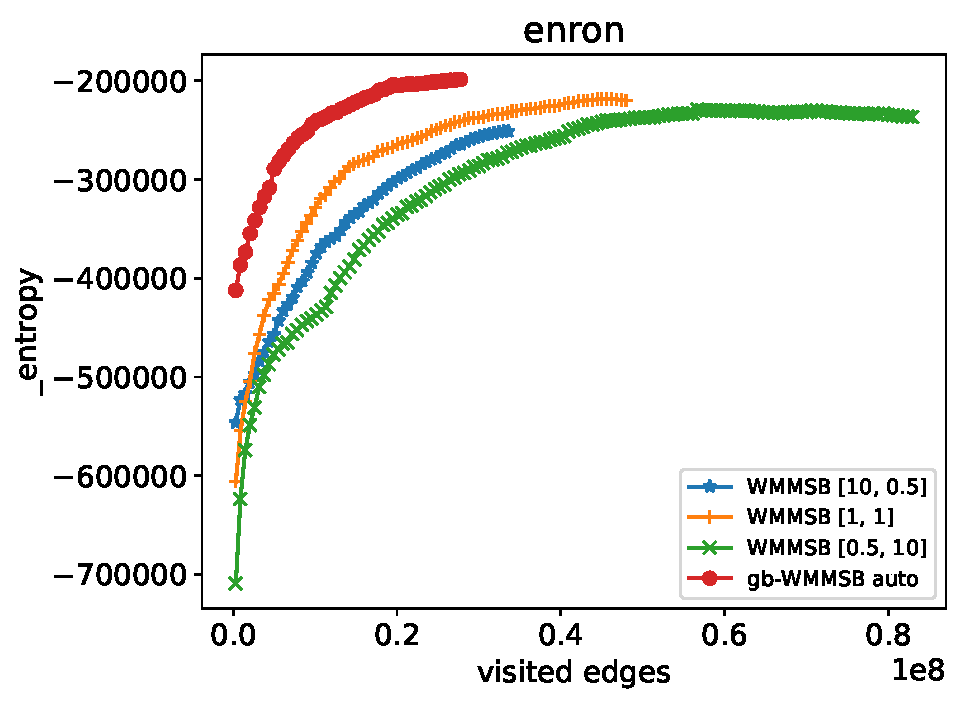
\includegraphics[width=0.32\textwidth]{warm2/enron_fig__entropy}
\end{subfigure}
\begin{subfigure}
         \centering
      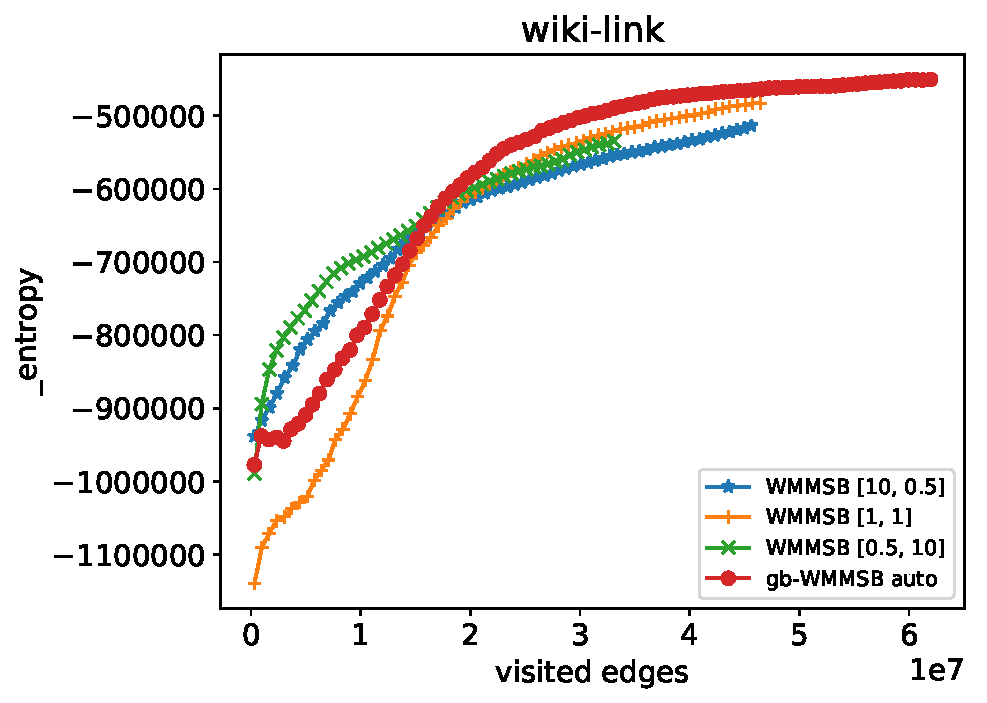
\includegraphics[width=0.32\textwidth]{warm2/wiki-link_fig__entropy}
\end{subfigure}
\begin{subfigure}
         \centering
      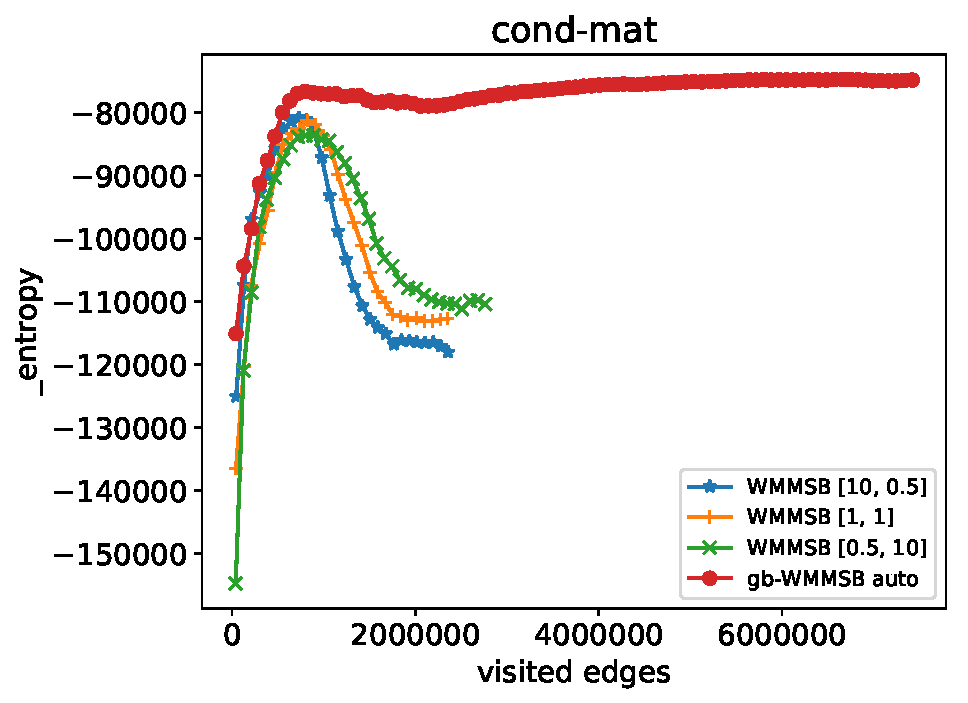
\includegraphics[width=0.32\textwidth]{warm2/cond-mat_fig__entropy}
\end{subfigure}
\caption{Log-likelihood convergence for WMMSB for different gamma prior. The bg-WMMSB model converges faster compared to fixed Gamma settings.}

    \label{fig:conv_entropy}
\end{figure}

\begin{equation*}
\log p(\D_{test}) = \sum_{i,j \in \D_{test}} \log p(y_{ij} | \phih_{kk'}) p(k|\thetah_i) p(k'|\thetah_j)
%\log p(\D_{test}) = \sum_{i,j \in \D_{test}} \log p(y_{ij} | \phih_{kk'}) p(k|\thetah_i) p(k'|\thetah_j)
\end{equation*}


%
% ROC
%

We evaluate the capacity of the models to predict missing links with the ROC-AUC curve on the testset. For the weighted models, the measure consists to evaluate to what extent they can reconstruct the topology of the network and to compare them with binary models. Thus, for the WMMSB models we compute the probability of observing a link as the probability to generate at least one edge count,

\begin{table}
\centering
	
\caption{AUC-ROC performance comparaison for two different size of testsets. In the top table, the testsets contains 20 percent of the edges. In the bottom table the testsets contains 80 percent of the edges. Score are averaged on 10 independants runs and for each run we randomly build the testsets that were held-out during the inference. For the SCVB inference, we fix the sampling parameter $m=50$.}

\begin{tabular}{llllll}
\toprule
$t_{ratio}=0.2$             &   MMSB &   WMMSB & bg-WMMSB      &    SBM &   WSBM \\
\midrule

 astro-ph                & 0.735 $\pm$ 0.018   & 0.717 $\pm$ 0.013    & 0.739 $\pm$ 0.004         & 0.676 $\pm$ 0.049 & 0.729 $\pm$ 0.062 \\
 cond-mat                & 0.675 $\pm$ 0.007   & 0.612 $\pm$ 0.019    & 0.662 $\pm$ 0.032         & 0.728 $\pm$ 0.045 & 0.752 $\pm$ 0.054 \\
 hep-th                  & 0.682 $\pm$ 0.008   & 0.659 $\pm$ 0.008    & 0.689 $\pm$ 0.009         & 0.672 $\pm$ 0.036 & 0.616 $\pm$ 0.036 \\
 netscience              & 0.684 $\pm$ 0.03    & 0.586 $\pm$ 0.04     & 0.724 $\pm$ 0.029         & 0.733 $\pm$ 0.077 & 0.774 $\pm$ 0.057 \\
 manufacturing           & 0.900 $\pm$ 0.003   & 0.884 $\pm$ 0.01     & 0.886 $\pm$ 0.006         & 0.876 $\pm$ 0.014 & 0.659 $\pm$ 0.052 \\
 fb\_uc                  & 0.820 $\pm$ 0.105   & 0.883 $\pm$ 0.004    & 0.871 $\pm$ 0.009         & 0.807 $\pm$ 0.019 & 0.662 $\pm$ 0.017 \\
 enron                   & 0.640 $\pm$ 0.159   & 0.849 $\pm$ 0.016    & 0.844 $\pm$ 0.021         & 0.562 $\pm$ 0.048 & 0.498 $\pm$ 0.088 \\
 wiki-link & 0.522 $\pm$ 0.12    & 0.723 $\pm$ 0.107    & 0.779 $\pm$ 0.016         & 0.615 $\pm$ 0.043 & 0.553 $\pm$ 0.047 \\

\bottomrule
\end{tabular}

\begin{tabular}{llllll}
\toprule
$t_{ratio}=0.8$             &   MMSB &   WMMSB & bg-WMMSB      &    SBM &   WSBM \\
\midrule

 astro-ph                & 0.729 $\pm$ 0.011   & 0.708 $\pm$ 0.008    & 0.739 $\pm$ 0.006         & 0.462 $\pm$ 0.046 & 0.617 $\pm$ 0.09  \\
 cond-mat                & 0.647 $\pm$ 0.01    & 0.601 $\pm$ 0.013    & 0.635 $\pm$ 0.015         & 0.474 $\pm$ 0.077 & 0.553 $\pm$ 0.04  \\
 hep-th                  & 0.652 $\pm$ 0.007   & 0.646 $\pm$ 0.004    & 0.631 $\pm$ 0.019         & 0.446 $\pm$ 0.053 & 0.457 $\pm$ 0.057 \\
 netscience              & 0.613 $\pm$ 0.011   & 0.580 $\pm$ 0.015    & 0.611 $\pm$ 0.018         & 0.470 $\pm$ 0.009 & 0.462 $\pm$ 0.013 \\
 manufacturing           & 0.883 $\pm$ 0.006   & 0.864 $\pm$ 0.008    & 0.851 $\pm$ 0.012         & 0.805 $\pm$ 0.023 & 0.654 $\pm$ 0.036 \\
 fb\_uc                  & 0.789 $\pm$ 0.104   & 0.857 $\pm$ 0.006    & 0.852 $\pm$ 0.011         & 0.569 $\pm$ 0.072 & 0.459 $\pm$ 0.083 \\
 enron                   & 0.659 $\pm$ 0.204   & 0.825 $\pm$ 0.075    & 0.866 $\pm$ 0.012         & 0.489 $\pm$ 0.108 & 0.344 $\pm$ 0.071 \\
 wiki-link & 0.608 $\pm$ 0.186   & 0.678 $\pm$ 0.12     & 0.779 $\pm$ 0.025         & 0.281 $\pm$ 0.053 & 0.227 $\pm$ 0.043 \\

\bottomrule
\end{tabular}


\label{table:roc}
\end{table}

\begin{equation*}
p(y_{ij} \geq 1 | \Thetah, \Phih) = 1 - \sum_{kk'} \thetah_{ik} \thetah_{jk'} e^{\phih_{kk'}}
\end{equation*}

The performance results in table \ref{table:roc} show that WMMSB is able to infer the topology of the networks. Furthermore, it outperforms the baseline for networks where weights represents natural information such as for communication and hyperlinks networks. 
In the other hand, MMSB and WMMSB under SCVI inference shows that they can infer the network topology when only observing a small portion of the networks, which represents an advantage in terms of scalability or when only a sub-graph of the real data are available.

%
% Sim
%

%For the weighted models, we further measure the capacity to predict right edge counts with a $l_1$ distance between the real count of the test set and the expected count of the models 
%
%\begin{equation*}
%D_{l_1}(D_{test} ||  \{\Thetah, \Phih\}) = \sum_{i,j \in \D_{test}} | y_{ij} - \E[y_{ij}|\Thetah, \Phih] |
%\end{equation*}



%
%  Figure analysis and commment
%





\section{Conclusion}
\label{sec:concl}



\clearpage
%\bibliographystyle{unsrt}
%\bibliographystyle{apalike}
\bibliographystyle{alpha}
%\bibliographystyle{splncs04}
\bibliography{./a}

\clearpage
\appendix
\section{Supplementary material of \textit{Mixed-Membership Stochastic Block Models for Weighted Networks}}
\section{Derivation of the collapsed variational updates}

The derivation of the collapsed variational updates is first obtained by maximizing the ELBO w.r.t $\gamma_{ijkk'}$ with:
%
\begin{align*}
\frac{\partial \L_Z}{\partial \gamma_{ijkk'}} &= \frac{\partial }{\partial \gamma_{ijkk'}}  \sum_{Z^{-ij}}\sum_{k_1=1}^K\sum_{k_2=1}^K  q(Z^{-ij}) \gamma_{ijk_1 k_2} (\log p(Y, Z^{-ij}, z_{i\rightarrow j}=k_1, z_{i\leftarrow j}=k_2|\Omega)+ \\
& \qquad \log q(Z^{-ij}, z_{i\rightarrow j}=k_1, z_{i\leftarrow j}=k_2) )   \\
&= E_{q(Z^{-ij})}[ p(Y, Z^{-ij}, z_{i\rightarrow j}=k, z_{i\leftarrow j}=k'|\Omega))] + H[Z^{-ij}] -\log(\gamma_{ijkk'}) +1
\end{align*}
%
By equating this derivative to zero, one obtains the following update:
\begin{equation} \label{eq1}
\gamma_{ijkk'} \propto \exp E_{q(Z^{-ij})} [\log P(z_{i\rightarrow j}=k, z_{i\leftarrow j}=k' | Y^{-ij}, Z^{-ij}, \Omega) ]
\end{equation}
%
with  $P(z_{i\rightarrow j}=k, z_{i\leftarrow j}=k' | Y^{-ij}, Z^{-ij}, \Omega)$ being the collapsed Gibbs update of WMMSB, of the form:
%
\begin{align*}
P(z_{i\rightarrow j}=k, z_{i\leftarrow j}=k' |Y^{-ij}, Z^{-ij}, \Omega) \propto (n_{\rightarrow ik}^{\Theta^{-j}} + \alpha_k) (n_{\leftarrow jk}^{\Theta^{-i}} + \alpha_{k'}) \mathrm{NB}\left(y_{ij}; n^{Y^{-ij}}_{kk'} + r, \frac{p}{p\,n^{\Phi^{-ij}}_{\bm{.}kk'} + 1} \right)
\end{align*}
%
with count statistics given by the following equations:

%\begin{align} \label{eq:sss}
%    n^{\Theta}_{\rightarrow ik} &= \sum_{j, k'} \gamma_{ijkk'}        & n^{\Theta}_{\leftarrow jk'} &= \sum_{i, k} \gamma_{ijkk'}  \nonumber \\
%    n^{\Phi}_{xkk'} &= \sum_{ij:y_{ij}=x} \gamma_{ijkk'}  & n^{Y}_{kk'} &= \sum_{ij} y_{ij}\gamma_{ijkk'}
%\end{align}

\begin{align*}                                                                                                                                        
&n^{\Theta}_{\rightarrow ik} = \sum_j \delta(\zij=k)\\
&n^{Y}_{kk'} = \sum_{ij} y_{ij}\delta(\zij=k, \zji=k') \\
&n^{\Phi}_{\bm{.}kk'} = \sum_{ij} \delta( \zij=k, \zji=k') 
\end{align*}   

By applying a first order Taylor expansion on Eq.~\eqref{eq1}, following \cite{teh2007collapsed}, one obtains:

\begin{equation}
\gamma_{ijkk'} \propto (E_{q(Z^{-ij})}[n_{\rightarrow ik}^{\Theta^{-j}}] + \alpha_k) (E_{q(Z^{-ij})}[n_{\leftarrow jk}^{\Theta^{-i}}] + \alpha_{k'}) \mathrm{NB}\left(y_{ij}; E_{q(Z^{-ij})}[n^{Y^{-ij}}_{kk'}] + r, \frac{p}{p\,E_{q(Z^{-ij})}[n^{\Phi^{-ij}}_{\bm{.}kk'}] + 1} \right) \nonumber
\end{equation}

Finally, using a Gaussian approximation (as in \textit{e.g.} \cite{asuncion2009smoothing}), one can estimate the expectations $E_{q(Z^{-ij})}[n_{\rightarrow ik}^{\Theta^{-j}}], E_{q(Z^{-ij})}[n_{\leftarrow jk}^{\Theta^{-i}}]$ and  $E_{q(Z^{-ij})}[n^{\Phi^{-ij}}_{\bm{.}kk'}]$ with the counts defined in Eq. 2 of Section 3.1.

\section{Beta-Gamma updates}

In the WMMSB-bg model, the collapsed variational distribution takes the form:

\begin{equation*}
q(\Pi) = q(\Theta, \Phi|Z, R, P) q(Z)q(R)q(P)
\end{equation*}

The variational distribution for $r_{kk'}$ is taken in the Gamma family:  $q(r_{kk'}) = \textrm{Gamma}(a_{kk'},b_{kk'})$ for $1\leq k,k' \leq K$. The collapsed ELBO can thus be rewritten as:

\begin{align*}
\log p(Y) \geq \L_{Z,R,P} &= \E_{q}[\log p(Y, Z, R, P|\Omega)] + \textrm{H}[q(Z)] + \textrm{H}[q(R)] + \textrm{H}[q(P)] \\
                        &= \E_{q}[\log p(Y, Z)] + \textrm{H}[q(Z)] \\
                        &\qquad + \E_{q}[\log p(R|Y,Z,P)] + \textrm{H}[q(R)] \\
                        &\qquad +\E_{q}[\log p(P|Y,Z)] + \textrm{H}[q(P)] 
\end{align*}

\paragraph{Optimizing $\gamma_{ijkk'}$}

In the Beta-Gamma augmentation, the parameters $p$ and $r$ are marginalized in the update given by Eq.~\eqref{eq1}:
\begin{equation}
\gamma_{ijkk'} \propto \exp E_{q(Z^{-ij})} [\log E_{q(r_{kk'})}[E_{q(p_{kk'})}[ P(z_{i\rightarrow j}=k, z_{i\leftarrow j}=k' | Y^{-ij}, Z^{-ij}, \Omega) ] ] ] \nonumber
\end{equation}

By using a first order Taylor expansion, one obtains:

\begin{equation}
\gamma_{ijkk'} \propto (N_{\rightarrow ik}^{\Theta^{-j}} + \alpha_k) (N_{\leftarrow jk}^{\Theta^{-i}} + \alpha_{k'}) \mathrm{NB}\left(y_{ij}; N^{Y^{-ij}}_{kk'} + \E_{q}[r_{kk'}], \frac{\E_{q}[p_{kk'}]}{\E_{q}[p_{kk'}]\,N^{\Phi^{-ij}}_{\bm{.}kk'} + 1} \right) \nonumber
\end{equation}

\paragraph{Optimizing $r_{kk'}$}

We isolate the part of the ELBO than depends only on $r_{kk'}$ parameters ($a_{kk'}$ and $b_{kk'}$). Thus, we consider only the links that have been generated within the classes $k,k'$, denoted by $Y^{(kk')}$. Furthermore, as $y_{ij} \sim NB(r_{kk'}, p_{kk'})$ if $i$ is in class $k$ and $j$ in class $k'$, one has:

\begin{align*}
\L_{[r_{kk'}]} = \E_{q(r_{kk'})}[\log p(r_{kk'}|Y^{(kk')},Z^{(kk')},p_{kk'})] + \textrm{H}[q(r_{kk'})] \\
\end{align*}

By applying Bayes rules and dropping the normalizing term that does not depend on $r_{kk'}$, one gets:

\begin{align*}
\L_{[r_{kk'}]} &= \E_{q(r_{kk'})}[\log \left( p(Y^{(kk')}|Z^{(kk')}, r_{kk'}, p_{kk'}) p(r_{kk'}]) \right)] + \textrm{H}[q(r_{kk'})] \\
    &= \E_{q(r_{kk'})}[\log \left( \prod_{ij\in Y^{(kk')}} \dbinom{r_{kk'} + y_{ij}-1}{y_{ij}} (1-p_{kk'})^{r_{kk'}} p_k^{y_{ij}} p(r_{kk'}) \right) ] + \textrm{H}[q(r_{kk'})] \\
    &= \E_{q(r_{kk'})}[\log \left( (1-p_{kk'})^{r_{kk'} N^{\Phi}_{kk'}} p_{kk'}^{N^{Y}_{kk'}} p(r_{kk'}) \prod_{ij\in Y^{(kk')}} \frac{\Gamma(r_{kk'}+y_{ij})}{\Gamma(r_{kk'}) \Gamma(y_{ij}+1) }  \right) ] + \textrm{H}[q(r_{kk'})]
\end{align*}

If $y_{ij} = 0$, then $\frac{\Gamma(r_{kk'}+y_{ij})}{\Gamma(r_{kk'}) \Gamma(y_{ij}+1)} = 1$, whereas if $y_{ij} \ne 0$, then $\frac{\Gamma(r_{kk'}+y_{ij})}{\Gamma(r_{kk'}) \Gamma(y_{ij}+1)} = \frac{1}{B(r_{kk'}, y_{ij})y_{ij}}$. Furthermore, in this latter case:
%
\begin{align*}
B(r_{kk'}, y_{ij}) = \int_0^1 t^{r_{kk'}-1} (1-t)^{y_{ij}-1} dt  \leq \int_0^1 t^{r_{kk'}-1} dt = \frac{1}{r_k}
\end{align*}
%
so that:
%
\begin{equation*}
\log \prod_{ij\in Y^{(kk')}} \frac{\Gamma(r_{kk'}+y_{ij})}{\Gamma(r_{kk'}) \Gamma(y_{ij}+1) } \geq N^Y_{kk'} \log(r_{kk'}) + \mathrm{cst}
\end{equation*}
%
with $N^Y_{kk'} = \sum_{ij\in Y^{(kk')}} y_{ij}$.

Furthermore, from the model definitions, one has: $\log p(r_{kk'}) = (r_0 c_0-1)\log(r_{kk'}) - r_{kk'} c_0 + \mathrm{cst}$  and $\textrm{H}[q(r_{kk'})] = a_{kk'} + \log(b_{kk'}) +\log \Gamma(a_{kk'}) + (1-a_{kk'})\Psi(a_{kk'})$.

Hence:
%
\begin{align*}
\L_{[r_{kk'}]} &\geq N^\Phi_{kk'} a_{kk'} b_{kk'} \log(1-p_{kk'}) + (r_0 c_0-1 )(\Psi(a_{kk'}) + \log(b_{kk'})) -c_0 a_{kk'} b_{kk'} +N^Y_{kk'} (\Psi(a_{kk'}) + \log(b_{kk'}))  \\
&\qquad a_{kk'} + \log(b_{kk'}) +\log \Gamma(a_{kk'}) + (1-a_{kk'})\Psi(a_{kk'})
\end{align*}

Maximizing the right-hand term of the above inequality with respect to $b_{kk'}$ yields:

\begin{equation} \label{eq:update2}
b_{kk'} = \frac{r_0 c_0 + N^Y_{kk'}}{a_{kk'} (c_0 - N^\Phi_{kk'} \log(1-p_{kk'}))} \nonumber
\end{equation}

As $r_{kk'} \sim \textrm{Gamma}(a_{kk'},b_{kk'})$, one finally obtains:

\begin{equation}
\E_q[r_{kk'}] = a_{kk'} b_{kk'} = \frac{r_0 c_0 + N^Y_{kk'}}{c_0 - N^\Phi_{kk'} \log(1-p_{kk'})} \nonumber
\end{equation}

\paragraph{Optimizing $p_{kk'}$}

In oder to maximize the ELBO w.r.t $p_{kk}'$, one can let $q(p_{kk'}) = p(p_{kk'} | Y,Z) = E_q(r_{kk'}) [ p(p_{kk'} | Y^{(kk')},Z^{(kk')} ,r_{kk'})]$. As the negative binomial and Beta distributions are conjugate, a closed-form expression can be obtained:

\begin{align*}
p(p_{kk'} | Y^{(kk')}, Z^{(kk')}, r_{kk'}) &\propto p(Y^{(kk')| Z^{(kk')}, r_{kk'}} p(r_{kk'}) \\
                               &\propto (1-p_{kk'})^{r_{kk'} N^\Phi_{kk'}}p_{kk'}^{N^Y_{kk'}} p_{kk'}^{c\epsilon -1} (1-p_{kk'})^{c(1-\epsilon) -1}\\
                               &\propto p_{kk'}^{c\epsilon + N^Y_{kk'} -1} (1-p_{kk'})^{c(1-\epsilon) + N^\Phi_{kk'}r_{kk'}-1}\\
                               &= \mathrm{Beta}(c\epsilon + N^Y_{kk'}, c(1-\epsilon) + N^\Phi_{kk'}r_{kk'})
\end{align*}

Finally, by resorting again to a first order Taylor expansion, one obtains:

\begin{equation*}
p_{kk'} \sim \mathrm{Beta}(c\epsilon + N^Y_{kk'}, c(1-\epsilon) + N^\Phi_{kk'} E_q[r_{kk'}]) \nonumber
\end{equation*}


%\section{Stratified Sampling}
%
%Sampling from minibatches in SVI, for MMSB model, was initially proposed in [6] and [7]. The adaptation of the sampling scheme for SCVI is based on the reformulation of the "sufficient statistics" $N^\Theta, N^\Phi$ and $N^Y$  by bringing up a minibatch distribution $h(S)$. The idea of the stratified sampling is to divide the edges into subset that share some statistical strength.
%For each node $n$ with divide it's neighbors pairs into a set $S_1$ containing all its links (edges) and a subset $S_0$ dividing into  $m$ set containing its non-links. Then sampling consists of drawing one of its its set $S_0$ or $S_0$ with probability.
%
%\begin{align*}
%h(S)=\begin{cases}
%    \frac{1}{2 N}  & \textrm{ if } S = S_1 \\
%    \frac{1}{2 N m}  & \textrm{ if } S \in S_0 
%    \end{cases}
%\end{align*}
%
%
%By referencing any of the global "sufficient statistics" of the models with the term $N^*$ such that $N^* \in \{N^Y, N^\Theta, N^\Phi\}$. Assuming that every pair (i, j) occurs in some constant number of sets c, $N^*$ can be reformulated as follows 
%
%\begin{align*}
%N^* = \sum_{ij, *} \gamma_{ij} = \E_h[ \frac{1}{c}\frac{1}{h(S)} \sum_{ij \in S, *} \gamma_{ij}  ]
%\end{align*}
%
%Where $N^*$ and $\gamma_{ij}$ are matricies of size $K\times K$.
%The exact summing formulation of $N^*=\sum_{ij,*}$ is given in section 3.1. For undirected network, $c$ is equal to 2 because each pair occurs in two set, and $c$ is 1 for directed network.


\section{Experimentation}

We provide here the complete set of results for the AUC-ROC scores evaluations for the full range of training sets proportions (1\%, 5\%, 10\%, 20\%, 30\%, 50\% and 100\%) in Figure \ref{fig:roc} for all the datasets. The log-likelihood convergence of the inference for all the datasets are given in Figure \ref{fig:conv_entropy},

\begin{figure}[h]
\centering
	

\begin{subfigure}
     \centering
         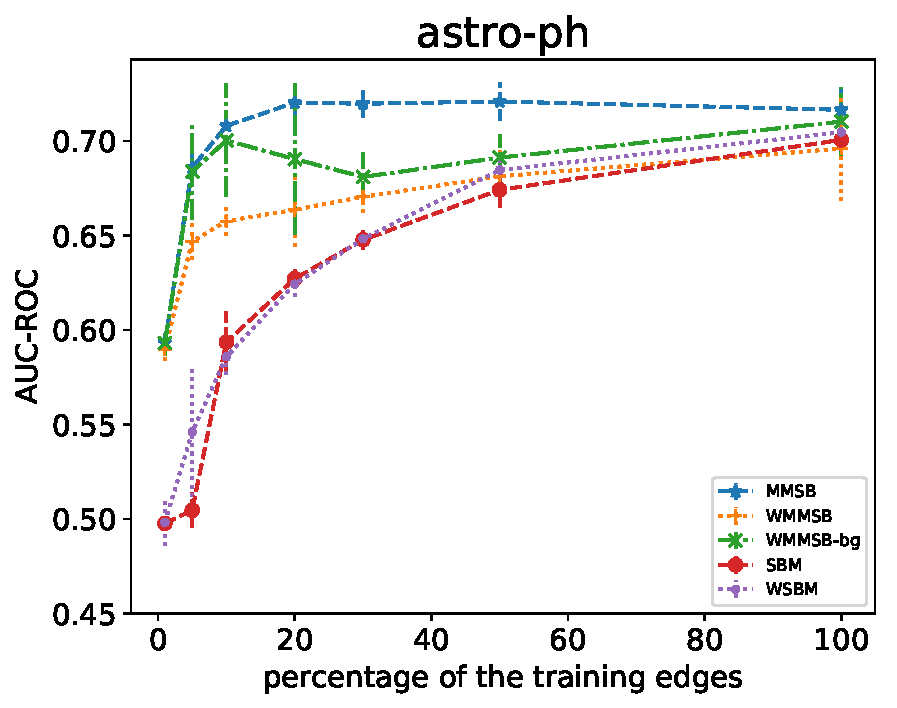
\includegraphics[width=0.32\textwidth]{fig/astro-ph__entropy@_roc_evo}
\end{subfigure}
\begin{subfigure}
         \centering
      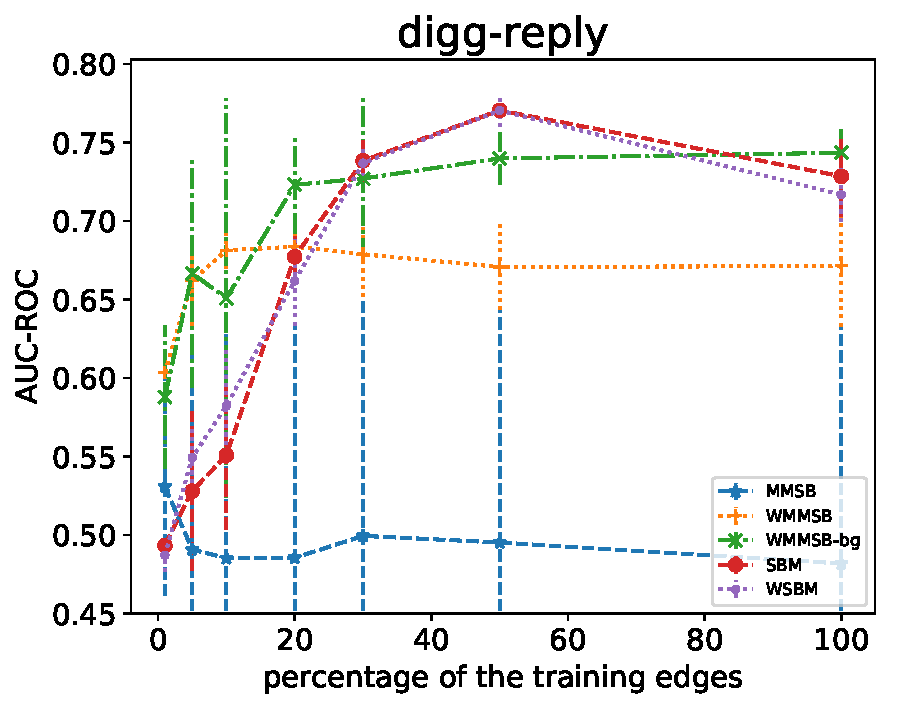
\includegraphics[width=0.32\textwidth]{fig/digg-reply__entropy@_roc_evo}               
\end{subfigure}                                                                          
\begin{subfigure}                                                                        
         \centering                                                                      
      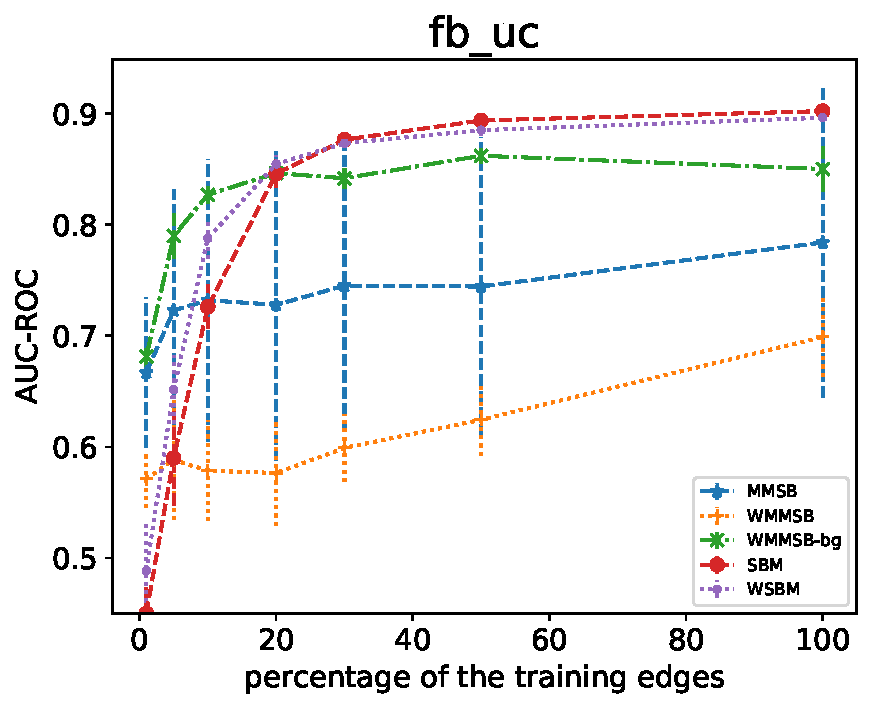
\includegraphics[width=0.32\textwidth]{fig/fb_uc__entropy@_roc_evo}
\end{subfigure}                                                                          
\begin{subfigure}                                                                        
         \centering                                                                      
      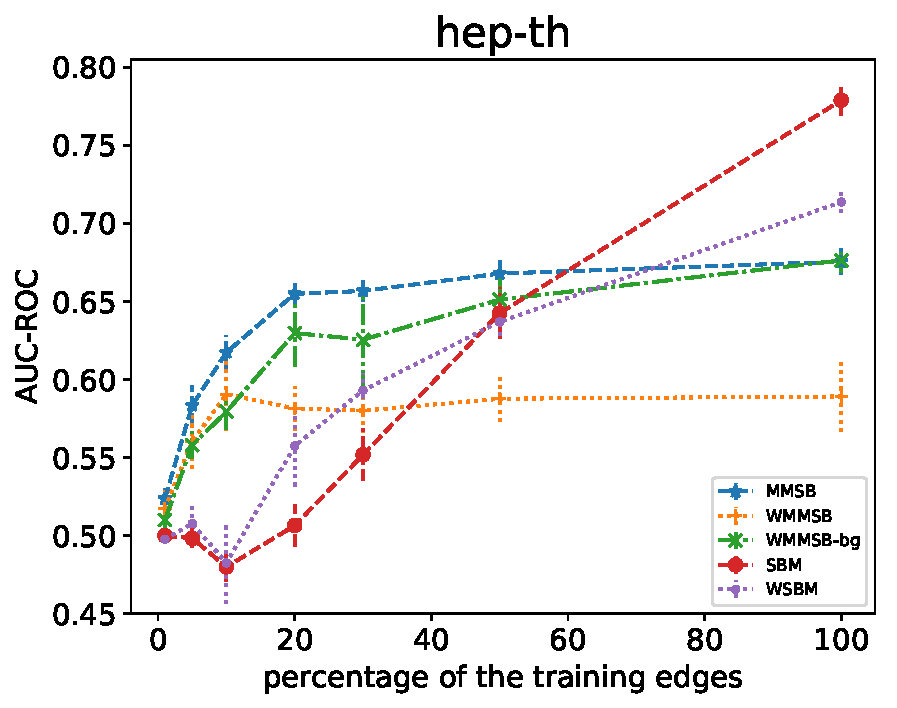
\includegraphics[width=0.32\textwidth]{fig/hep-th__entropy@_roc_evo}
\end{subfigure}                                                                          
\begin{subfigure}                                                                        
     \centering                                                                          
         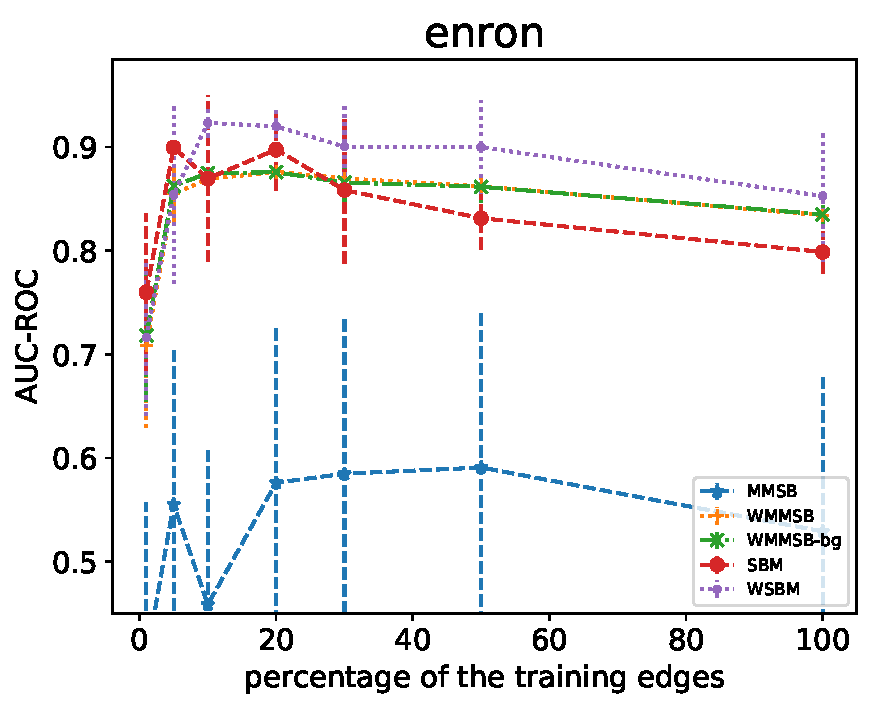
\includegraphics[width=0.32\textwidth]{fig/enron__entropy@_roc_evo}
\end{subfigure}
\begin{subfigure}
         \centering
      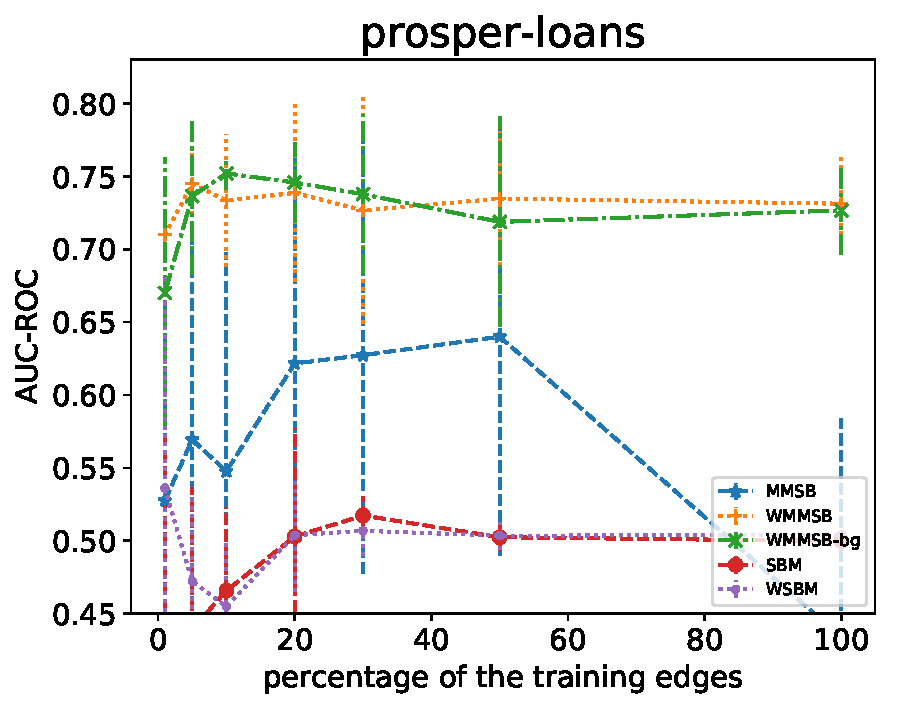
\includegraphics[width=0.32\textwidth]{fig/prosper-loans__entropy@_roc_evo}
\end{subfigure}                                                             
\begin{subfigure}                                                           
         \centering                                                         
      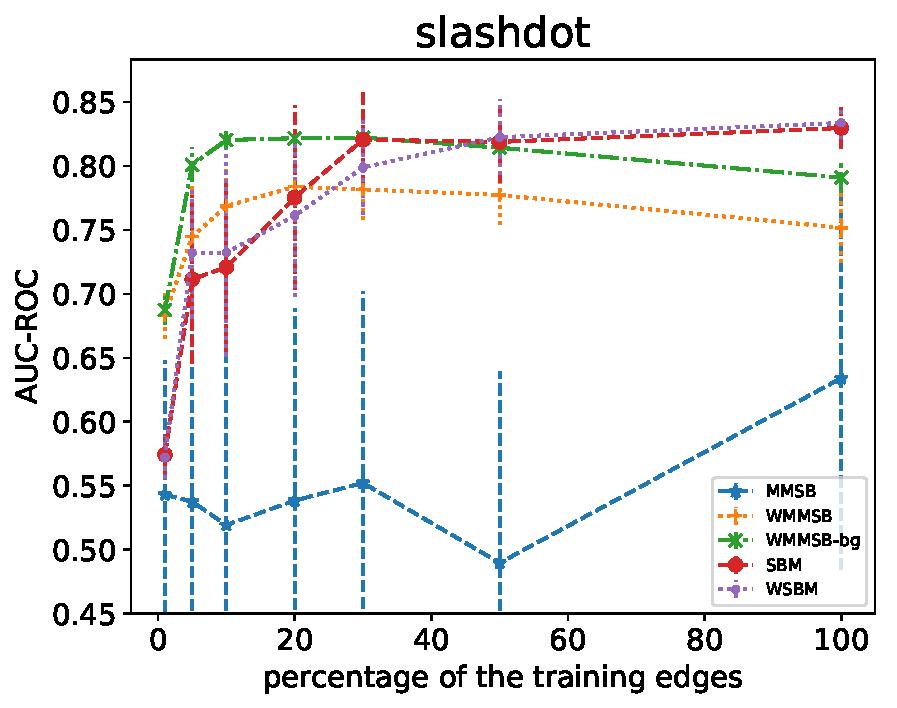
\includegraphics[width=0.32\textwidth]{fig/slashdot__entropy@_roc_evo}
\end{subfigure}                                                             
\begin{subfigure}                                                           
         \centering                                                         
      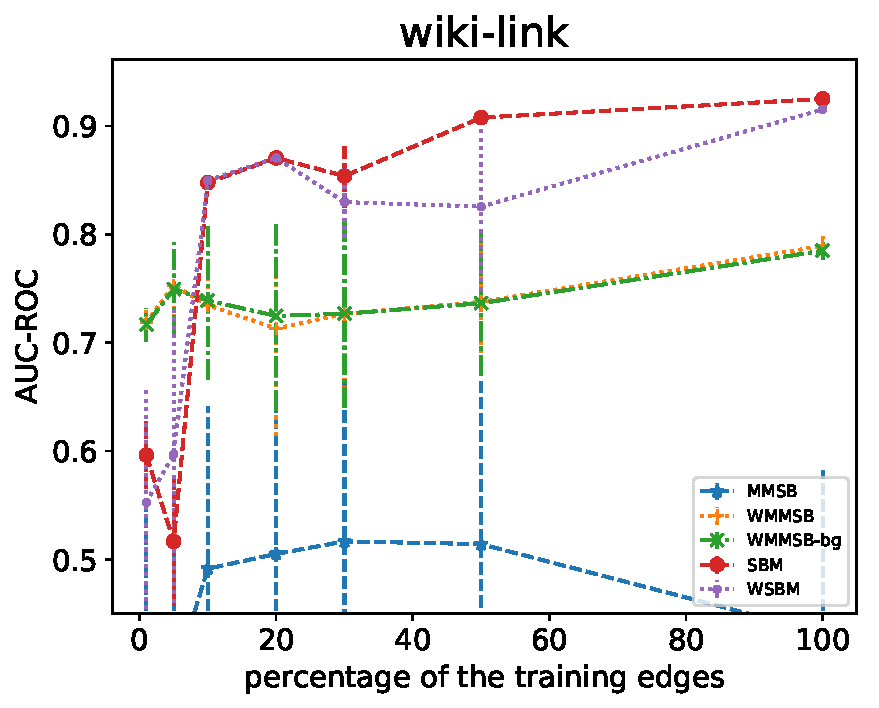
\includegraphics[width=0.32\textwidth]{fig/wiki-link__entropy@_roc_evo}
\end{subfigure}                                                             
\begin{subfigure}                                                           
         \centering                                                         
      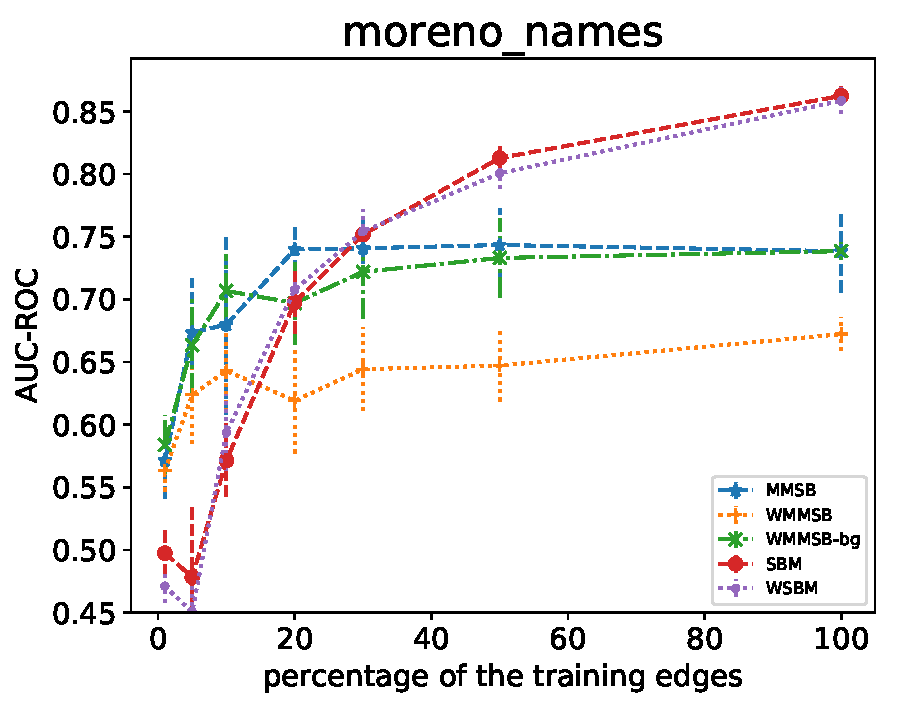
\includegraphics[width=0.32\textwidth]{fig/moreno_names__entropy@_roc_evo}
\end{subfigure}                                                             
\caption{Comparison of models in terms of AUC-ROC scores according to the percentage of edges used to train the models (from 1 to 100\%).}


   \label{fig:roc}
\end{figure}


\begin{figure}[h]
\centering
	
\begin{subfigure}
     \centering
         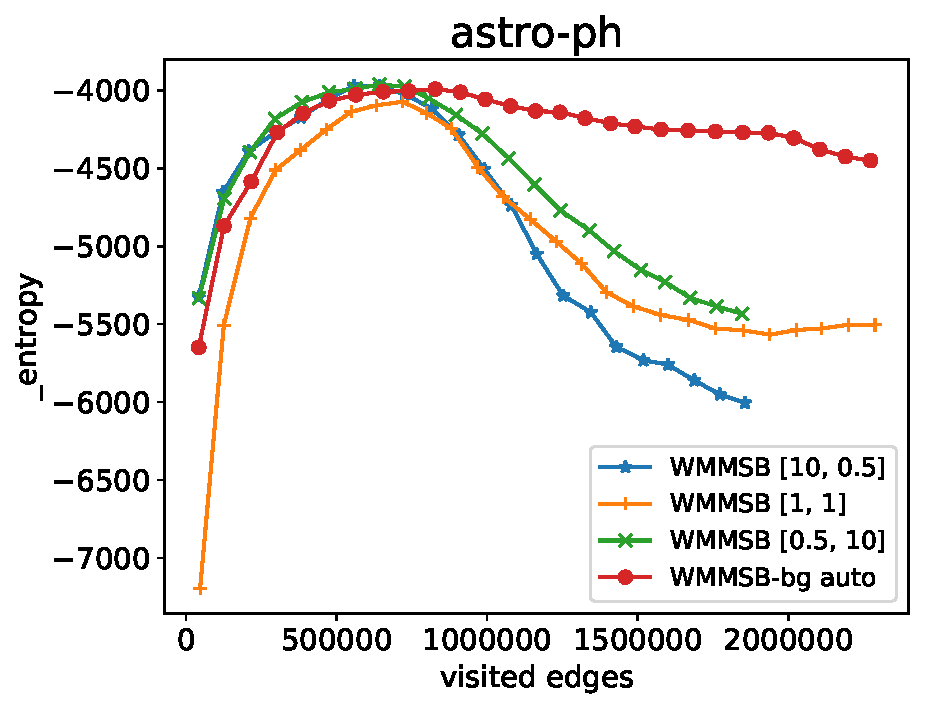
\includegraphics[width=0.32\textwidth]{fig/astro-ph_fig__entropy}
\end{subfigure}
\begin{subfigure}
         \centering
      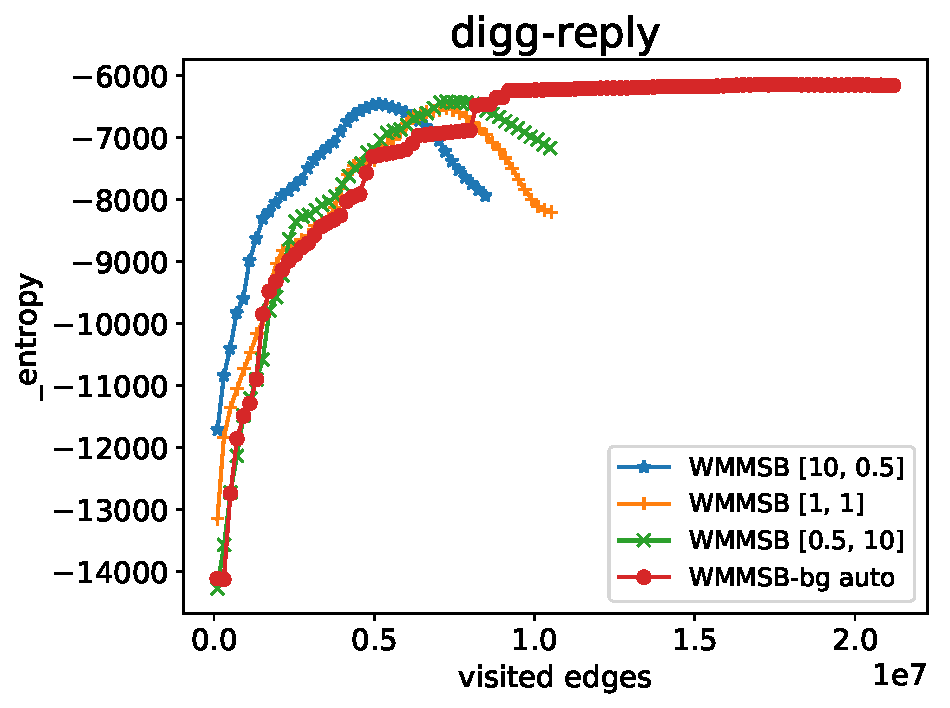
\includegraphics[width=0.32\textwidth]{fig/digg-reply_fig__entropy}               
\end{subfigure}                                                                          
\begin{subfigure}                                                                        
         \centering                                                                      
      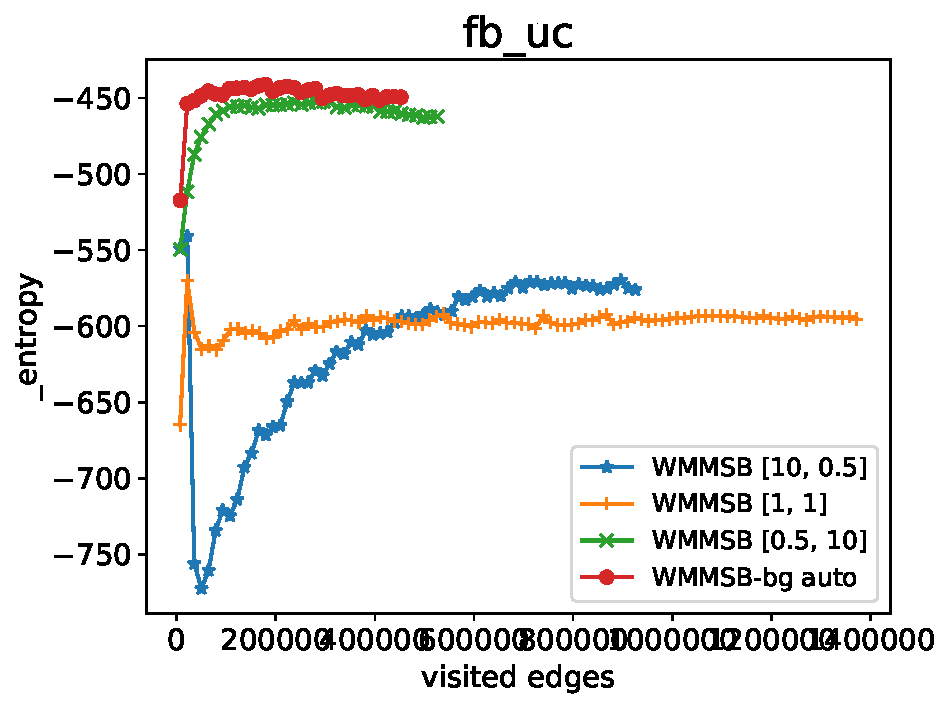
\includegraphics[width=0.32\textwidth]{fig/fb_uc_fig__entropy}
\end{subfigure}                                                                          
\begin{subfigure}                                                                        
         \centering                                                                      
      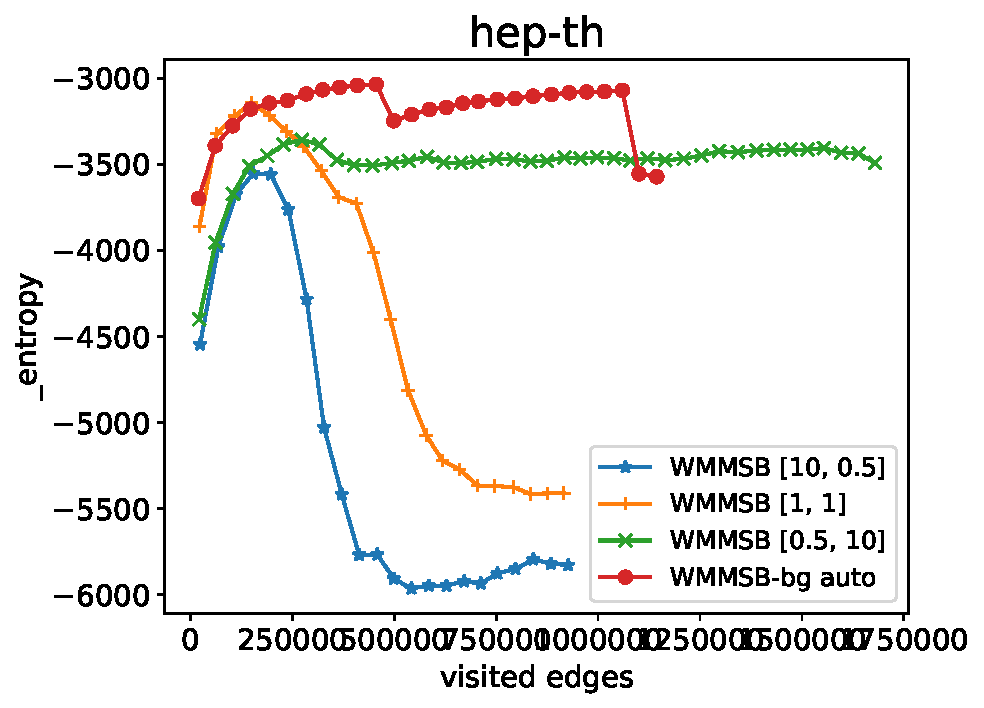
\includegraphics[width=0.32\textwidth]{fig/hep-th_fig__entropy}
\end{subfigure}                                                                          
\begin{subfigure}                                                                        
     \centering                                                                          
         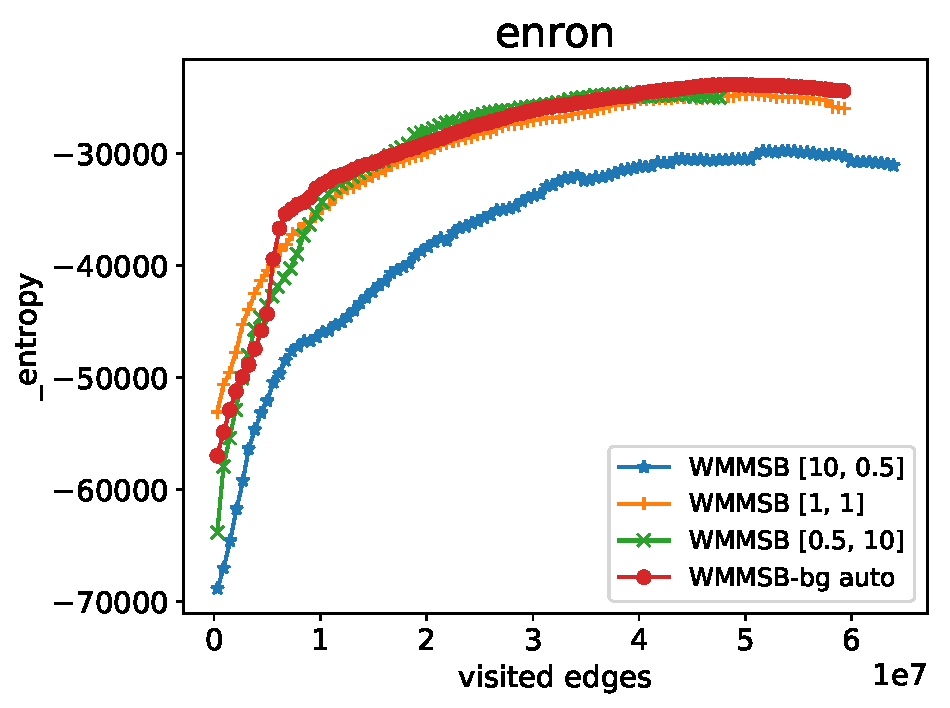
\includegraphics[width=0.32\textwidth]{fig/enron_fig__entropy}
\end{subfigure}
\begin{subfigure}
         \centering
      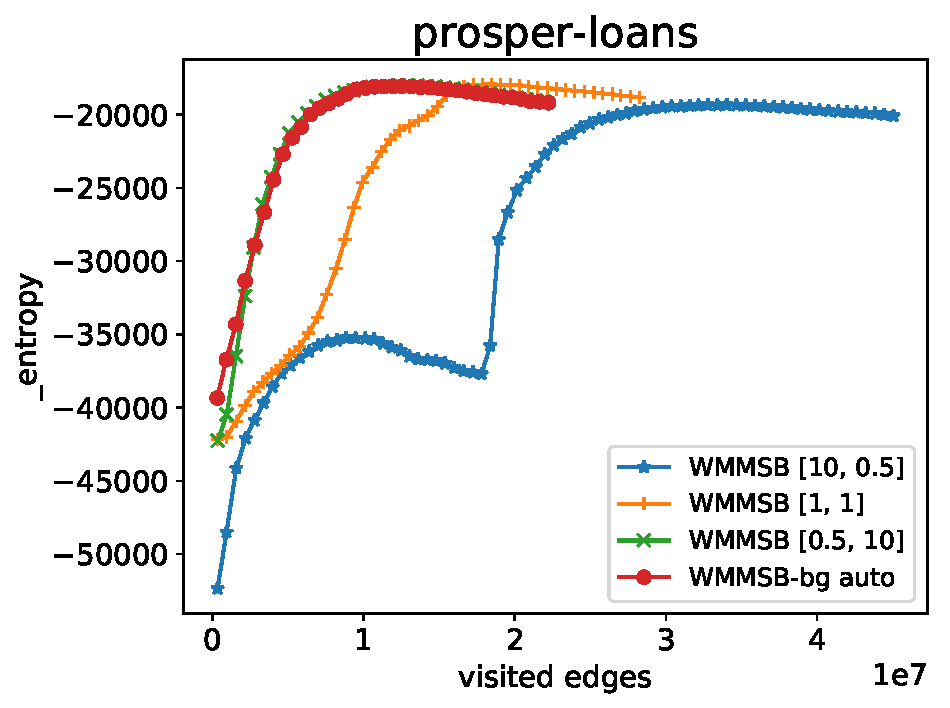
\includegraphics[width=0.32\textwidth]{fig/prosper-loans_fig__entropy}
\end{subfigure}                                                             
\begin{subfigure}                                                           
         \centering                                                         
      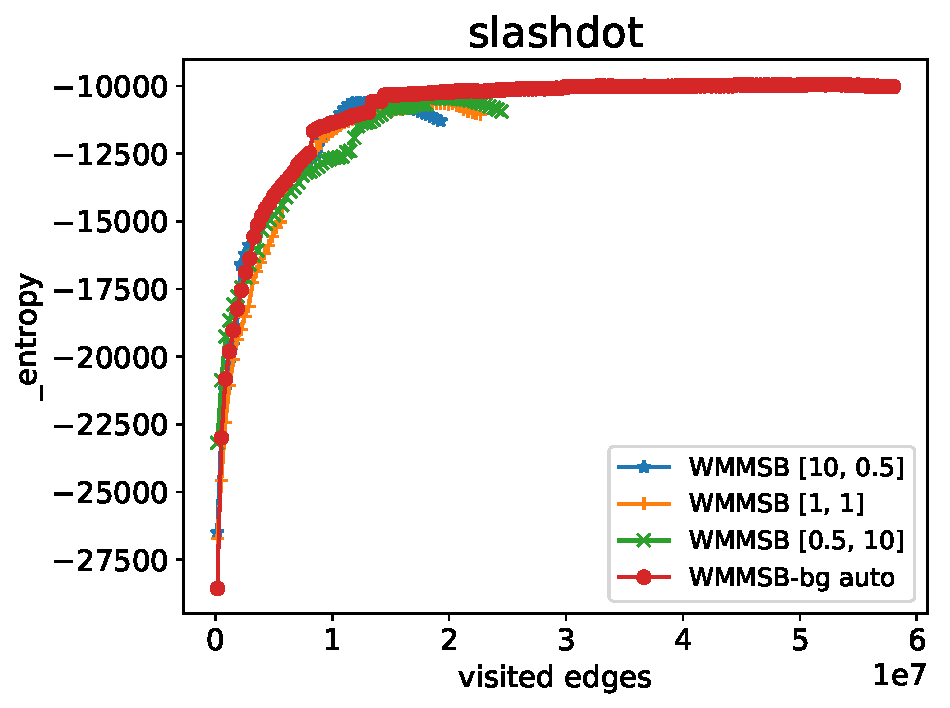
\includegraphics[width=0.32\textwidth]{fig/slashdot_fig__entropy}
\end{subfigure}                                                             
\begin{subfigure}                                                           
         \centering                                                         
      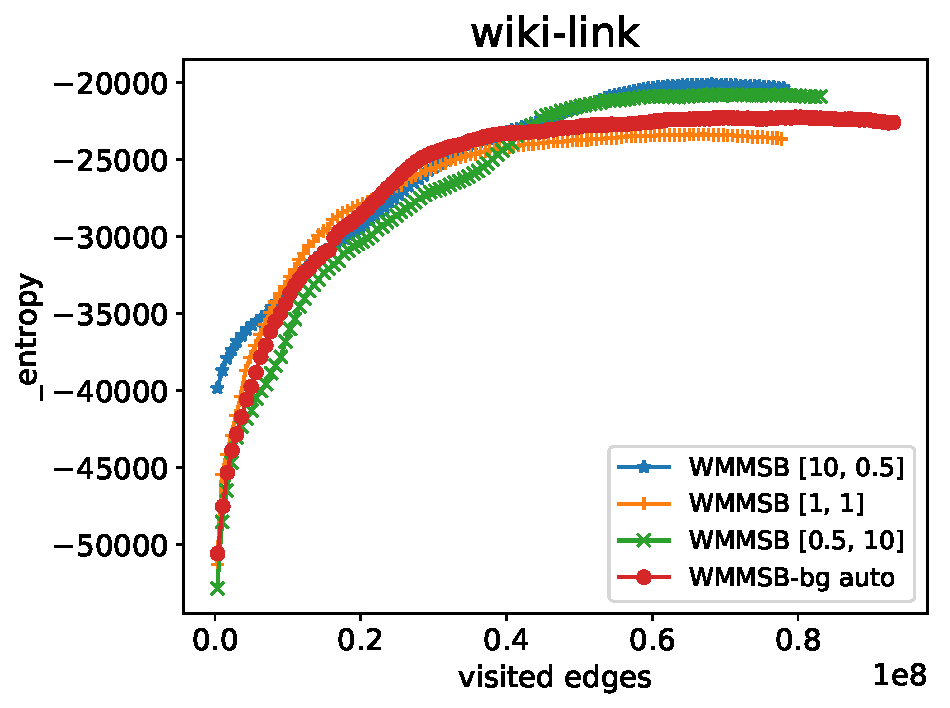
\includegraphics[width=0.32\textwidth]{fig/wiki-link_fig__entropy}
\end{subfigure}                                                             
\begin{subfigure}                                                           
         \centering                                                         
      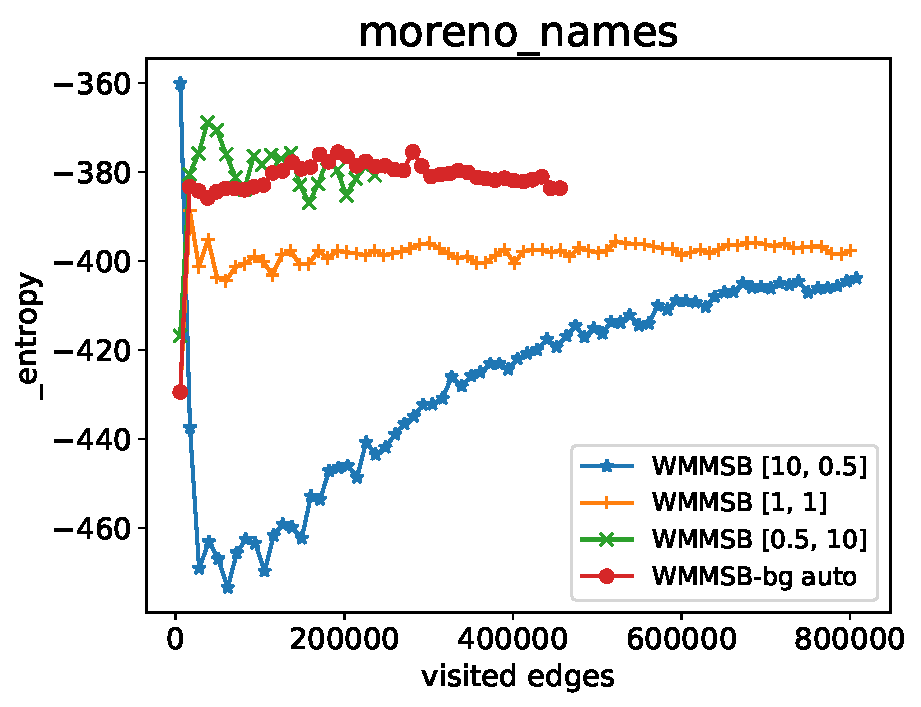
\includegraphics[width=0.32\textwidth]{fig/moreno_names_fig__entropy}
\end{subfigure}                                                             
\caption{Log-likehood convergence for WMMSB and WMMSB-bg models. Three different sets of hyper-parmeter are used for WMMSB.}


    \label{fig:conv_entropy}
\end{figure}

\section{Reproducible Research}

We published our implementation within a platform that aims to ease the development of reproducible complex experiments. We are maintaining this platform that we released under open-source license.\footnote{The name of the project is anonymized.}

To reproduce our results, one can proceed as follows:
\begin{itemize}
\item Install the XXX project:   %\lstinline|git clone https://github.com/*/XXX|  
    \begin{lstlisting}[language=bash]
          $ git clone https://github.com/*/*
          $ cd XXX and make install
    \end{lstlisting}
\item Fit all the models on all the corpus, and save the results:
\begin{lstlisting}[language=bash]
        $ XXX online_roc -x fit -w --repeat 0 1 2 3 4 5 6 7 8 9 
\end{lstlisting}
\item Parallelization can be obtained by adding the options \lstinline|--cores NUMBER_OF_CORES|,
\item Figures can be plotted with the command:  
\begin{lstlisting}[language=bash]
        $ XXX online_roc -x roc_evolution2 --repeat 0 1 2 3 4 5 6 7 8 9
\end{lstlisting}
\end{itemize}



\end{document}
